\chapter{Computational Study}
\label{chap:Melcomp}

\begin{itquote}{}
You don't really understand what you've got \\
until you do a comprehensive model of it.
\end{itquote}

\begin{flushright}
Christopher Tyler \\ 
(Q\&A session at VSS 2019)
\end{flushright}

\textit{The work presented here has been presented previously as a poster presentation at VSS 2018 \citep{garside_does_2018}\footnote{Poster available: \doi{10.6084/m9.figshare.6280865.v1}}, a poster presentation at the Visual Neuroscience Summer School (Rauischholzhausen 2018), and as an oral presentation at ICVS 2019 \footnote{Slides and abstract available: \doi{10.6084/m9.figshare.8832395.v1}}}.

\section{Summary}

A computational study was performed to explore whether a melanopsin signal would be useful for colour constancy in a real world environment, and to reduce the search space for future psychophysical experiments. This research was exploratory in nature (as opposed to confirmatory) with the goal being a furthering of our understanding of the problem and generation of hypotheses, rather than the confirmation of specific hypotheses \citep{steinle_entering_1997}.

It was found that an additional receptor with a spectral sensitivity different from that of the cone receptors was able to deliver a signal which could effectively be used to transform input signals to an illuminant-independent space. 

The spectral sensitivity of melanopsin was found to be optimal for this task, though only to the extent that whilst a number of different spectral positionings would provide a valuable signal, a sensor with the spectral sensitivity of melanopsin performs slightly better than the rest.

Notably, this type of algorithm makes no assumptions about scene-level attributes (in the way that \acrlong{GW} and \acrlong{BiW} do).

% I am interested in the question of whether a melanopic signal might be useful for either estimating the illuminant(s) in a scene, or more directly transforming visual signals into an illuminant-independent space.

% Following initial psychophysical experiments, where results did not indicate a strong or simple relationship, I chose to take a step back and examine the problem that the HVS is faced with in a natural environment, which colour constancy solves. Through this route I hoped to answer the questions:
% \begin{enumerate}
% 	\item Would it be sensible for the HVS to use a melanopic signal to help solve this problem?
% 	\item If so, in what way would it be used?
% \end{enumerate}

Code is provided: \url{https://github.com/da5nsy/Melanopsin_Computational}

\section{Introduction}

In the other chapters of this thesis the approach taken to study the effect of melanopsin has mirrored standard practice: we think that melanopsin \emph{might} be involved in a specific process and so we run an experiment where we vary the amount of melanopsin activation within a stimulus (our independent variable) and measure something to see if there is an associated change in the target dependent variable, with the hope of understanding \emph{how} melanopsin might be involved in the target process, but at no point do we really drill down on the questions of \emph{why} melanopsin might be involved in this process.

This has meant that it is unclear whether our results (positive or negative) can be taken at face value - perhaps our baseline assumptions about how or why melanopsin is involved were wrong, and we were consequently looking in the wrong place.

This chapter describes an exploratory computational study which took an ecological modelling approach to further our understanding of what, if any, benefits may arise by the use of a melanopsin-based signal for colour constancy.

\noindent The proposed benefits of this approach are: 
\begin{enumerate}
    \item It may be possible to answer the question of whether it is sensible for melanopsin to be involved in colour constancy in any form whatsoever - is there any benefit to be gained from involving melanopsin?
    \item We may be able to suggest or rule out specific computational structures - one computation might be beneficial whilst others might not be.
    \item It may help to narrow the search area for future psychophysical experimentation - in previous experiments there have been lots of assumptions about the luminance range over which melanopsin is active, the spatial distribution (both in terms of receptive fields and influence over signals from distant parts of the retina), the temporal dynamics of the signals involved (and many other assumptions but conscious and unconscious). This is an opportunity to test whether a melanopsin-based signal is useful for specific ranges of the stimulus space.
\end{enumerate}

\noindent The key research question for this section can be posed thus:

\begin{quote}
\centering 
Considering the conditions on our planet, \\
and the ecological requirements of vision, \\
would a signal from a melanopsin-expressing cell \\
be useful for colour constancy?
\end{quote}

This chapter will describe the computational investigation and accompanying thought process in roughly chronological order.

\section{Data sources}

\subsection{Illuminant and Surface Data Sources}

A useful guide to some of the existing datasets has been provided by \citet{kohonen_databases_2006}, though many of the links have rotted since publication, some new datasets have become available, and some datasets that weren't included have become known to me. In this section I shall describe the datasets available for use in studies such as this.

\subsubsection{Daylight datasets}

It is standard practice (see for example \citet{barrionuevo_contributions_2014}) to use illuminants generated from from CIE D-series formulae (see \gls{PTB} function `GenerateCIEDay') which are derived data collected by \citet{judd_spectral_1964}. Whilst the D-series provides a good approximation of daylight spectra, empirical data better represents any link between chromaticity and luminance, and any bias in the likelihood of occurrence of one spectrum over another. It is thought that the original data of Judd et al. is no longer available \citep[p.~60]{maloney_computational_1984}. The first three principal components of the data are available through \gls{PTB} as `B\_cieday'.

\paragraph{Granada Data.}
The Granada daylight database \citep{hernandez-andres_color_2001} contains 2600 measurements of daylight taken over the course of two years at a single site in Granada, Spain. Data is recorded for 300-1100nm with sampling interval of 5nm.\footnote{This data has been made available at \url{http://colorimaginglab.ugr.es/pages/Data}}

\paragraph{Other sources.}

The Parkkinen and Silfsten data described by \citet{kohonen_databases_2006}\footnote{Available at \url{http://cs.joensuu.fi/spectral/databases/download/daylight.htm}} comprises 14 measurements of daylight from afternoon and evening. The wavelength range is 390nm - 1070nm, with 4nm intervals.

The other potential sources of data, in addition to the \citet{judd_spectral_1964} data, do not seem to be currently available, but for completeness I provide them here: \citet{condit_spectral_1964, tarrant_spectral_1968, dicarlo_illuminant_2000, taylor_distribution_1941, henderson_spectral_1964, sastri_typical_1968, dixon_spectral_1978, sastri_spectral_1966,williams_statistical_2009,bui_group_2004}.

There are two authoritative reference books on the subject: \citet{henderson_daylight_1970,henderson_daylight_1977} (first and second editions) and \cite{robinson_solar_1966}. Also of interest may be \citet{minnaert_light_1993} (various editions), and \citet{lynch_color_2001} (various editions).

Two further datasets which are available only upon request are held by Dr Andrew Smedley of The Univesity of Manchester (320nm to 2800nm, since 2010, data collection ongoing) and Marina Khazova of Public Health England\footnote{Minimally described here: \url{https://uk-air.defra.gov.uk/research/ozone-uv/uv-uk-monitoring}} (350nm - 830nm, 1nm interval). It is hoped that these datasets may be made openly available at some point in the future.

Data specifically for dawn and dusk (with a small amount of data extending into what could be considered `daylight' is available from \citet{spitschan_variation_2016} as open access supplementary material from the journal publisher. 

An interesting additional source of data may be the work of \citet{peyvandi_colorimetric_2016}, who simulate a very large number of daylight, sunlight and skylight spectra. 

Finally, there is also a large corpus of information specifically about the light conditions in forest environments, although I have not yet had opportunity to investigate whether collected datasets have been made available \citep{sumner_catarrhine_2000,chiao_characterization_2000,federer_spectral_1966,geiger_climate_2003,thery_forest_2001,xu_changes_2013,wang_real-time_2006,endler_color_1993,brinkmann_light_1971,de_castro_light_2000,freyman_spectral_1968,fassnacht_review_2016,blackburn_seasonal_1995}.

%hutchison_relighting_2009

\subsubsection{Surface Reflectance datasets}

\paragraph{Krinov data.}
The Krinov data was originally published in 1947 \citep{krinov_spektralnaya_1947}, though it is now mainly accessed through a Canadian translation published a few years later \cite{krinov_spectral_1953}. It has recently been made available through \gls{PTB} \cite{brainard_psychophysics_1997} (as sur\_krinov.mat), and forms part of the SFU dataset \cite{barnard_data_2002}. It consists of 370 measurements of natural surfaces, measured at 9 locations around the USSR. It includes a large number of repeated measures (generally of objects at different angles), and has many measurements of objects which might be described as `background' surfaces rather than objects per se (e.g. soil, sand, turf). Measurements are available at 10nm sampling interval, mostly between 400 and 650nm, with some extending as far as 900nm, and some without data at parts of the range. The \gls{PTB} version of the data is a reduced set of 191 measurements, having excluded a number of measurements of various types of grass. 

\paragraph{`Natural Colors' data.}
The `Natural Colors' data \citep{parkkinen_spectral_1988} was collected to allow investigators to explore how well reflectances could be represented by low dimensional models\footnote{It is available at: \url{http://www.uef.fi/web/spectral/natural-colors}}. The data consists of 219 reflectance spectra of different leaves and flowers, between 400 and 700nm with interval of 5nm. It has recently been made available through \gls{PTB} (as sur\_koivisto.mat).

\paragraph{Vrhel et al. data.}
The \citet{vrhel_measurement_1994} data in its complete form comprised measurements of 64 Munsell chips, 120 Du Pont paint chips and 170 natural and non-natural objects. Similarly to the `Natural Colors' data, this data was again collected to allow investigations into the dimensionality of natural refelctance functions. The authors noted that they aimed to improve upon the Krinov data by decreasing the sampling interval (to 2nm), increasing the range of objects measured (and focusing on more object-like objects as opposed to background objects) and increasing the sampling range (to 390-730nm). To my knowledge only part of this set is currently available, as the FTP server referenced in the original publication is no longer accessible. The object reflectances alone are available through \gls{PTB} (as `sur\_vrhel.mat').

\paragraph{Standard Object Colour Spectra Database for Colour Reproduction Evaluation (SOCS) data.}
This international standard \citep{tajima_development_1998,iso/tc_130_graphic_technology_iso/tr_2003} collates more than 50,000 spectral reflectances of a wide range of type of surfaces, grouped into several categories. The database was originally created in order to allow for the assessment of colour reproduction of image input devices. Unfortunately, this data proves very difficult to access, and as yet I have been unable to assess it.

\paragraph{NASA data.}
The NASA data-set \citep{david_e._bowker_spectral_1985} comprises 156 measurements of different terrains and materials, presented to aid in the design of remote imaging systems to optimally detect surfaces of interest and to detect changes over time in these surfaces where this is of interest (e.g. changes in spectral signatures that reveal growth or disease of specific crops). Data was not collected by the authors, but digitised from 58 different sources, and so range and interval are not consistent throughout the set. Whilst the authors seem to have devoted a great deal of energy and care to accurate digitisation, `digitisation' seems to be limited to the printing of tabulated values rather than provision of digital files (we've come a long way since 1985) and so any use of this data may need to start with an extended period of careful transcription. The surfaces chosen for this set are sensibly biased towards those of interest to remote sensing applications, and so use of this data in vision science would likely require careful consideration. It is expected that there may be other similar datasets tailored to the needs of remote sensing which may be available, should this type of data be appropriate.

\paragraph{Foster et al. hyperspectral images}
The hyperspectral images of \citet{nascimento_statistics_2002,foster_frequency_2006} provide nominal \glspl{SRF} for full natural and suburban scenes. This data is valuable and rich in many ways. 

Notably, it can begin to represent the ubiquity/rarity of certain types of reflectances in the natural world, whereas the statistical distribution of surface variability in the abstracted databases so far considered is at the mercy of the collator. As Maloney puts it: ``in sampling spectral reflectances, we weight each spectral reflectance by its frequency of occurrence under whatever selection procedure we choose'' \cite{maloney_computational_1984}.

Additionally, the spatial inter-relationships between surfaces can be considered, which may be of particular value in trying to understand how an organism might operate under real-world conditions.

\begin{figure}[htbp]
    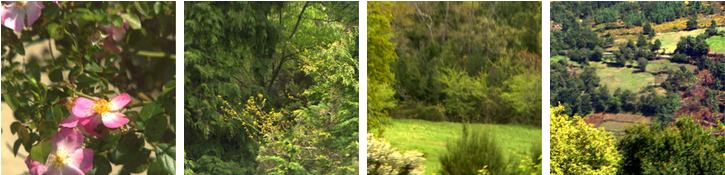
\includegraphics[max width=\textwidth]{figs/LitRev/Foster.png}
    \caption{A visualisation of the hyperspectral data for the first four images of the \citet{nascimento_statistics_2002} data. The other four available images are of non-natural environments.}
    \label{fig:Foster}
\end{figure} 

%In many ways hyperspectral images represent the ideal data for this type of experiment. They are much more closely linked to the real-world challenges faced by the human visual system in terms of statistical and spatial distribution of reflectances than data comprising abstracted spectral reflectances of a selected range of sampled surfaces. The statistical distribution of surface variability in an abstracted database is at the mercy of the collator, as Maloney puts it: ``in sampling spectral reflectances, we weight each spectral reflectance by its frequency of occurrence under whatever selection procedure we choose''\cite{maloney_computational_1984}. Of course the individual scenes still need to be selected in some way, with implicit assumptions about the goals of the human visual system being baked in at this stage (for example - should scenes include grassy landscapes and flora, trees laden with fruit, predators in hiding or human skin tones?).
%Using two-dimensional images would also allow for more advanced chromatic adaptation models to be considered, such as the group of algorithms based on Weijer et al.'s `Grey Edge' ideas \cite{weijer_edge-based_2007}. 

However, caution must be taken when using such data; whilst the hyperspectral images available are nominally `reflectance' images, the way in which reflectance is computed may make them unsuitable for some uses. Reflectance is estimated from radiance images by assuming uniform illumination across the scene, which for some use cases may be a particularly problematic simplification. %This is an acceptably minor distinction for many use cases, but in this specific case this introduces error in precisely the place where it needs to be avoided. In considering the effectiveness of chromatic adaptation transforms the goal is to separate the effect of variable reflectance functions from variable power distributions, and the ability to do this is hindered if an element of the power distribution variability is baked into the reflectance functions.

One final dataset which is worth mentioning, but which does not currently appear to be easily accessible: the `494 natural surfaces contain leaves, petals, grasses and barks' mentioned by \citet{cheung_color_2004} and further described by \citet{macdonald_realistic_2014}. It is hoped that this dataset may be made openly available in the future.

%'Natural Minolta' %Note: referenced in kohonen_databases_2006 but I can't find anything else about it or access it anywhere

A final note here - whilst the use of spectral reflectance data from natural sources is often preferable to that from non-natural sources, it is possible that the careful use of non-natural data could be permitted following the finding of Maloney \cite{maloney_evaluation_1986} that basis elements derived from measurements of Munsell colour samples provide excellent fits to natural data (specifically, the Krinov data).

Going further, it may be possible in some cases to use entirely artificial data; \citet{chen_physical_2005} showed that an artificial dataset, generated following the physical constraints on real \glspl{SRF} (as discussed by \citet{nassau_physics_2001}), seems to strongly resemble real datasets.

\subsection{Chosen Data sources}

Foundational data consisting of 
a subset\footnote{Every 20th value (130 of total 2600), to reduce compute time, and increase legibility of plots.} of the Granada daylight dataset 
\citep{hernandez-andres_color_2001}\footnote{Data: \url{http://colorimaginglab.ugr.es/pages/Data\#__doku_granada_daylight_spectral_database}},
the Stockman-Sharpe 10$^{\circ}$ cone fundamentals 
\citep{stockman_spectral_2000,stockman_spectral_1999}
(aka the CIE 2006 10$^{\circ}$ cone fundamental sensitivity functions \cite{cie_cie_2006})\footnote{Available as `T\_cones\_ss10' in \gls{PTB}.},
the melanopsin fundamental of \citet{lucas_measuring_2014}\footnote{Available as `T\_melanopsin' in \gls{PTB}.},
and a subset\footnote{10 surfaces were chosen from the Vrhel dataset, with a roughly even representation of skin tones, fruit, and vegetable/greenery.} 
of the reflectances of \citet{vrhel_measurement_1994}\footnote{Available as `sur\_vrhel' in \gls{PTB}.}
were used.

Tristimulus values $[L,M,S]$ and analogous melanopic values $I$ (as per standard tristumulus values but using the melanopsin fundamental, see Equation \ref{eq:iMB}) were computed as per Equation \ref{eq:MBTristim} for each illuminant. A real-world version of this would be to measure a spectralon tile (or other uniformly reflective surface) under each daylight condition. Tristimulus values were then computed for each surface under each illuminant.

\gls{MB} chromaticity co-ordinates were calculated, for both illuminant alone and for each surface under each illuminant, as per Equation \ref{eq:MB}\footnote{Note to assist in the reading of associated code: the normalising factors $k$ were applied during the Equation \ref{eq:MB} rather than Equation \ref{eq:MBTristim}.} The \gls{MB} chromaticities are plotted in Figure \ref{fig:MB}. 

\bigskip
\noindent
Support for various other options was included:
\begin{itemize}
    \item A range of CIE D series illuminants\footnote{Generated with the \gls{PTB} function `GenerateCIEDay'.}
    \item Scenes 1-4 of the
\citet{nascimento_statistics_2002}\footnote{Data: \url{https://personalpages.manchester.ac.uk/staff/d.h.foster/Hyperspectral_images_of_natural_scenes_02.html}} hyperspectral reflectance data
    \item Scenes 1-5 of the 
\citet{foster_frequency_2006}\footnote{Data: \url{https://personalpages.manchester.ac.uk/staff/d.h.foster/Hyperspectral_images_of_natural_scenes_04.html}}
hyperspectral reflectance data
\end{itemize}

The CIE D-series illuminants allowed for a smaller and more controlled daylight dataset and the Nascimento/Foster et al. data allowed for a more realistic distribution of reflectances.

\begin{figure}[htbp]
    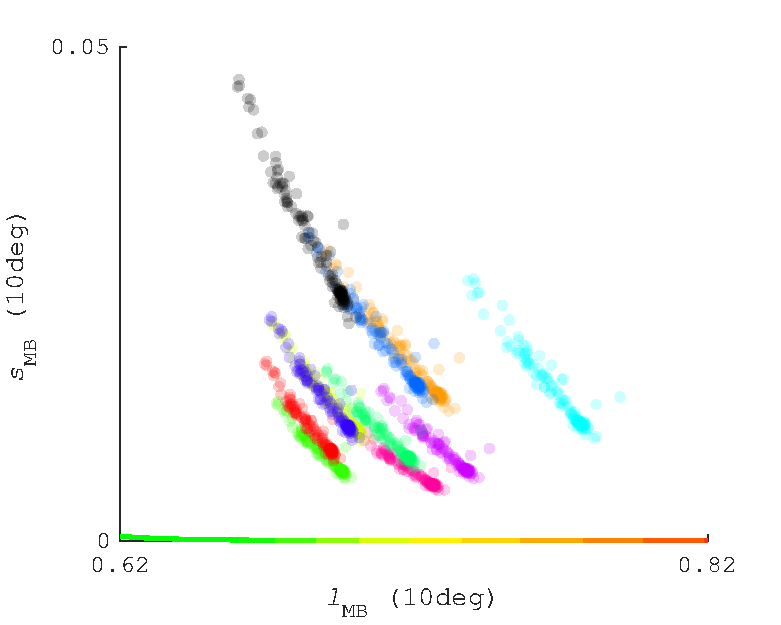
\includegraphics[max width=\textwidth]{figs/comp/predictingChromaticity/BasicMB_2.pdf}
    \caption{\gls{MB} chromaticities of 130 daylight illuminants (black points), and for 10 reflectances under each illuminant (coloured points). Colours not linked to surface appearances; they are arbitrary and used solely to distinguish different surfaces from one another). The edge of the spectral locus is visible along the lower edge.}
    \label{fig:MB}
\end{figure} 

% -------------------------- %

\section{Recovering the chromaticity of daylight}

The simplest computational method to achieve colour constancy is through normalisation of receptor signals by the hypothetical receptor signals to the illuminant. It is the implicit assumption in previous experiments that a melanopic signal could act as a cue to the chromaticity of the illuminant.

This is what \citet{maloney_physics-based_2001} refers to as the `RGB heuristic', and in some ways only delivers rough colour constancy, but it is nonetheless valuable. In most situations appearance of a scene under two different illuminants will be roughly relatable via the chromaticity of those illuminants.\footnote{However, it should be noted that there is no mathematical reason for this to be strictly true due to different colour rendering properties.}

\bigskip
\noindent
Initially, two questions were proposed:
\begin{enumerate}
\item Considering only daylight spectra (excluding reflective surfaces), can a melanopic signal predict the chromaticity of daylight? \item Now considering also object reflectances, can a melanopic signal predict the chromaticity of the daylight? 
\end{enumerate}

\subsection{First-level signals}

In this chapter the terminology of \citet{barrionuevo_contributions_2014} is employed; following their usage `first-level signals' are those which are direct photoreceptor catches (or analogues, such as $XYZ$ tristimulus values), and `second-level signals' are those computed by comparison of one signal with one or more other signals (such as $xy$ or \gls{MB} chromaticity values).

In order to visualise the relationship between the chromaticity of the illuminant and the resulting receptor catches, three-dimensional plots were made displaying $l_{\text{MB}}$ against $s_{\text{MB}}$ against $[L,M,S,I]$ in turn. \gls{MB} chromaticity space was chosen due to its status as a physiologically based chromaticity diagram, following the logic that if biologically plausible mechanisms are sought, then computations in a space best representing the real space are preferable. The plot for $I$ is shown in Figure \ref{fig:level1}. Other plots closely resembled this one. It can be seen that although there exists some relationship between the chromaticity values of the illuminants and the $I$ values, it does not appear as though one could be used reliably to predict the other. 

There is an almost bimodal relationship; all that can be gained from this relationship is the understanding that if the $I$ value is above a certain threshold, it is likely to be in a group with a relatively low $s_{\text{MB}}$ and relatively high $l_{\text{MB}}$ value. The real-world correlate of this is - \textit{if the daylight is bright enough, I can be fairly confident that the chromaticity of light will be relatively warm in colour.} This is as expected, since the brightest daylight conditions are likely to be those with unobstructed direct sunlight, which is warmer in \gls{CCT} than illumination provided by the blue sky. This relationship could not be used to predict the precise chromaticity of an illuminant. A near-identical trend is seen when surfaces are considered (the coloured points in Figure \ref{fig:level1}).

\begin{figure}[htbp]
    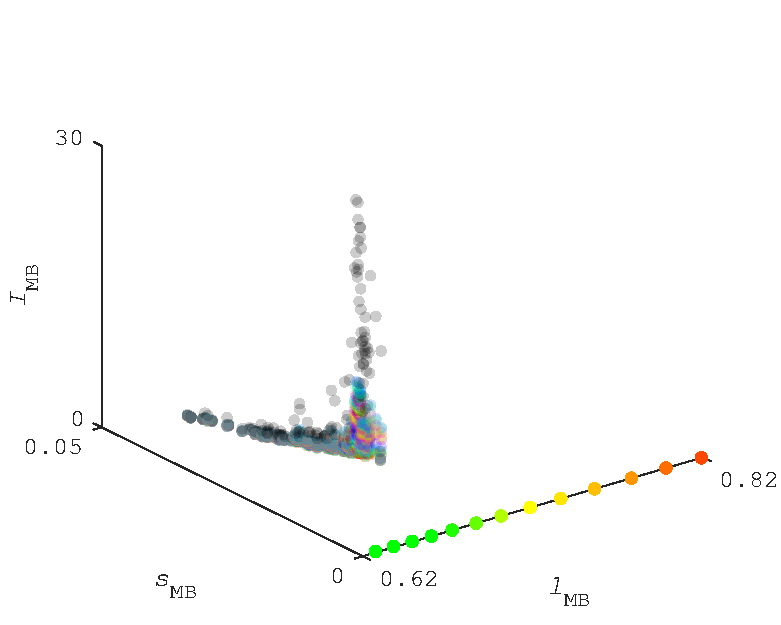
\includegraphics[max width=\textwidth]{figs/comp/predictingChromaticity/CvsI.pdf}
    \caption{\gls{MB} chromaticity of 130 illuminants plotting against the $I$ values for the illuminants alone (black points) and 10 different surfaces (coloured points). The edge of the spectral locus is visible along the $l_{\text{MB}}$ edge of the diagram.}
    \label{fig:level1}
\end{figure} 

\subsection{Second-level signals}
Following this, similar plots were made which plotted $l_{\text{MB}}$ against $s_{\text{MB}}$ as before, but now plotted the various second-level combinations of $[L,M,S,I]$, created by considering one signal divided by another (e.g. $L/M$), on the z-axis. These plots are shown in Figure \ref{fig:allComboSignals}. The plots created all showed clear and relatively simple relationships between chromaticity and these new derived signals, at least for the illuminant-only values. 

\begin{figure}
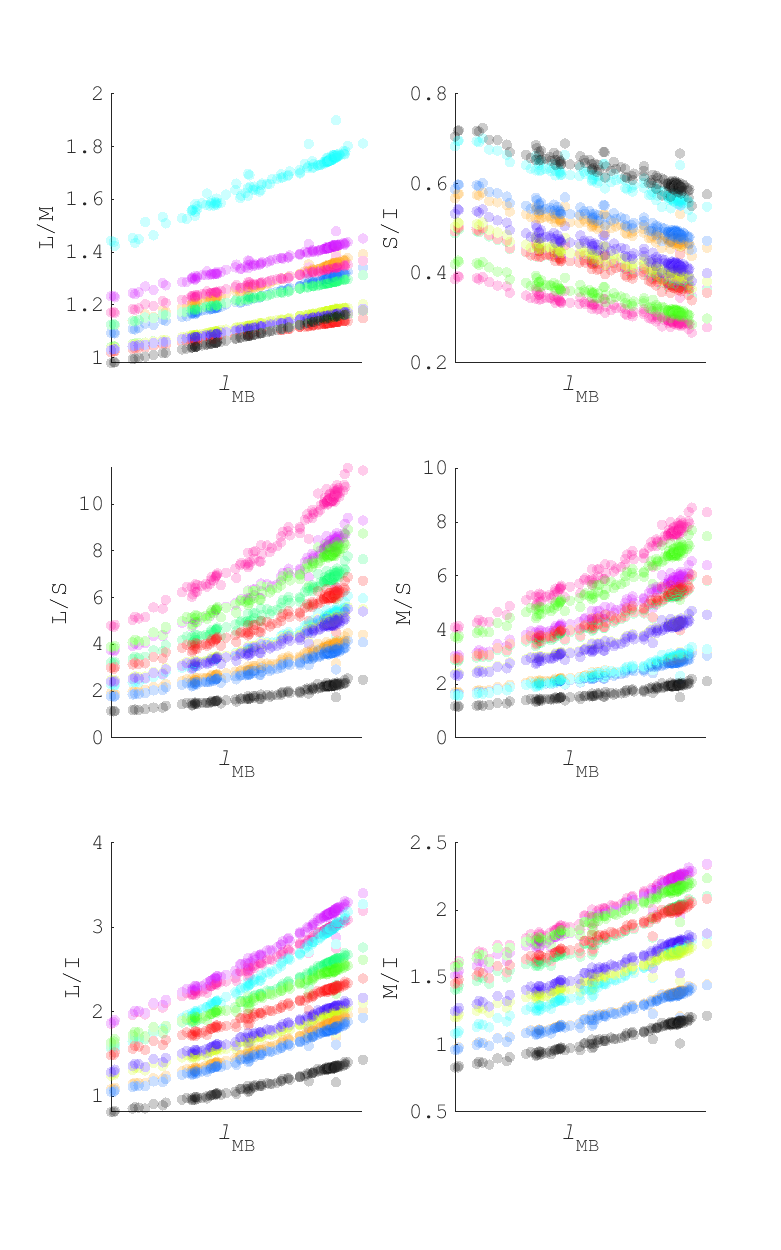
\includegraphics[max width=0.8\textwidth]{figs/comp/predictingChromaticity/allComboSignals.pdf}
\caption{Relationship between chromaticity and second-level signals. Plotted on the x-axis here is $l_{\text{MB}}$, with second-level signals on the apparent y-axis. During analysis these plots were three dimensional, with the apparent y-axis being a z-axis and the x-axis joined by a y-axis of $s_{\text{MB}}$. As before, black points indicate direct illuminant values, with coloured values corresponding to surface reflectances (though the colours do not relate the surfaces other than to distinguish one from another). It can be seen that on a per object basis (incl. no object) there is good correlation between chromaticity and all of the above signals. A similar relationship holds for the $s_{\text{MB}}$ perspective.}
% See gifs online at...
\label{fig:allComboSignals}
\end{figure}

A similar trend was seen for each individual surface as was seen for illuminant-only, however these relationships appear to be offset from that for a perfect reflector.

\subsection{A PCA interpretation}

These results seem to make intuitive sense if we consider the daylight dataset from a \gls{PCA} perspective (Figure \ref{fig:PCA})%\footnote{Note that weighting within the \gls{PCA} was given as following the outsides of the spectral sensitivity curves of s-cones and l-cones (both normalised to unity), and unity between their peaks. For a further discussion of this fiddly topic see \citet{maloney_evaluation_1986}.}
. For this dataset \gls{PC1} is broad and relatively smooth, and accounts for 99.888\% of the variance, and so a first-level signal in any part of the spectrum is going to essentially track this component. 

\begin{figure}[htbp]
 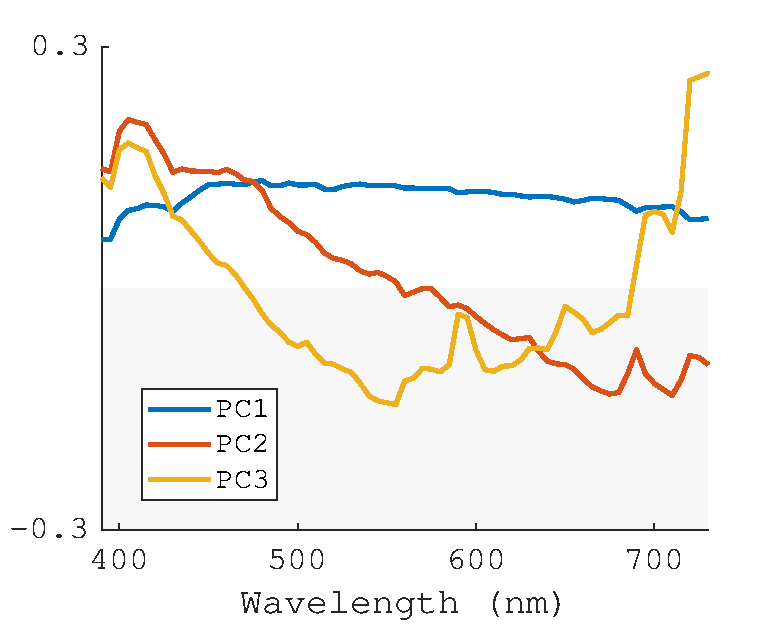
\includegraphics[max width=\textwidth]{figs/comp/melcomp_3/PC.pdf} %legend required
 \caption{The first 3 principal components for the Granada daylight dataset. These first three components account for 99.888\%, 0.077\% and 0.015\% of variance respectively.}
 \label{fig:PCA}
\end{figure} 

\Gls{PC2} is relatively smooth and monotonic (and accounts for 0.077\% of the variance). Almost any comparison between signals at different points in the spectrum (second-level signal) is going to roughly track this component (though the relative contribution of this component will slightly depend on the value of \gls{PC1}).

% Could add a plot relating chromaticity to PC2 and PC3 here.

Each surface will reflect different parts of the spectrum, meaning that this sampling of \gls{PC2} will vary from surface to surface, but the same overall trend will be followed.

%\begin{figure}[htbp]
%  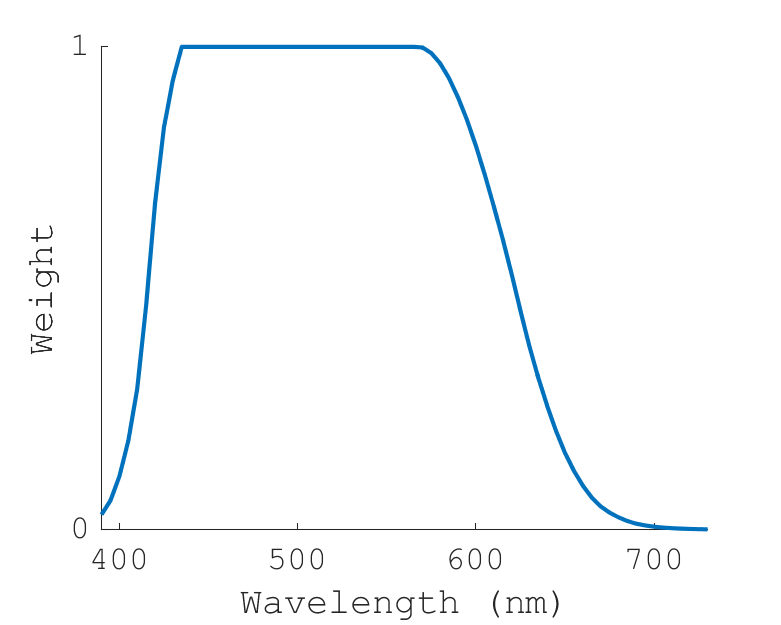
\includegraphics[max width=\textwidth]{figs/comp/melcomp_3/vw.png}
%  \caption{The variable weightings applied during the \gls{PCA} analysis. Generated by tracing the upward ramp of the S-cone sensitivity being used, plateauing at unity until the decrease of the L-cone sensitivity, and then following the decrease of the L-cone sensitivity.}
%  \label{fig:VW}
% \end{figure} 

\subsection{Relationships as artefacts}

For many of these signals however, such relationships are likely to arise solely from the manner in which each signal is constructed\footnote{My thanks go to Manuel Spitschan for convincing me of this point.}. For example, a relationship between $l_{\text{MB}}$ and $L/M$ might be expected, since $l_{\text{MB}}$ is defined as $L$ divided by the sum of weighted components of $L$ and $M$ (Equation \ref{eq:MB}). To confirm this, a control condition was performed, where $[L,M,S,I]$ was replaced by randomly generated values, and the second-level signals were generated as before. The results can be seen in Figure \ref{fig:allComboSignals_rand}. Relationships between secondary signals derived from $L$, $M$ or $S$ signals still showed correlations with chromaticity (albeit now points fell on a plane, instead of a line), whereas signals with an $I$ component showed only minimal coherence, forming a noisy cloud in three-dimensional space. 

\begin{figure}
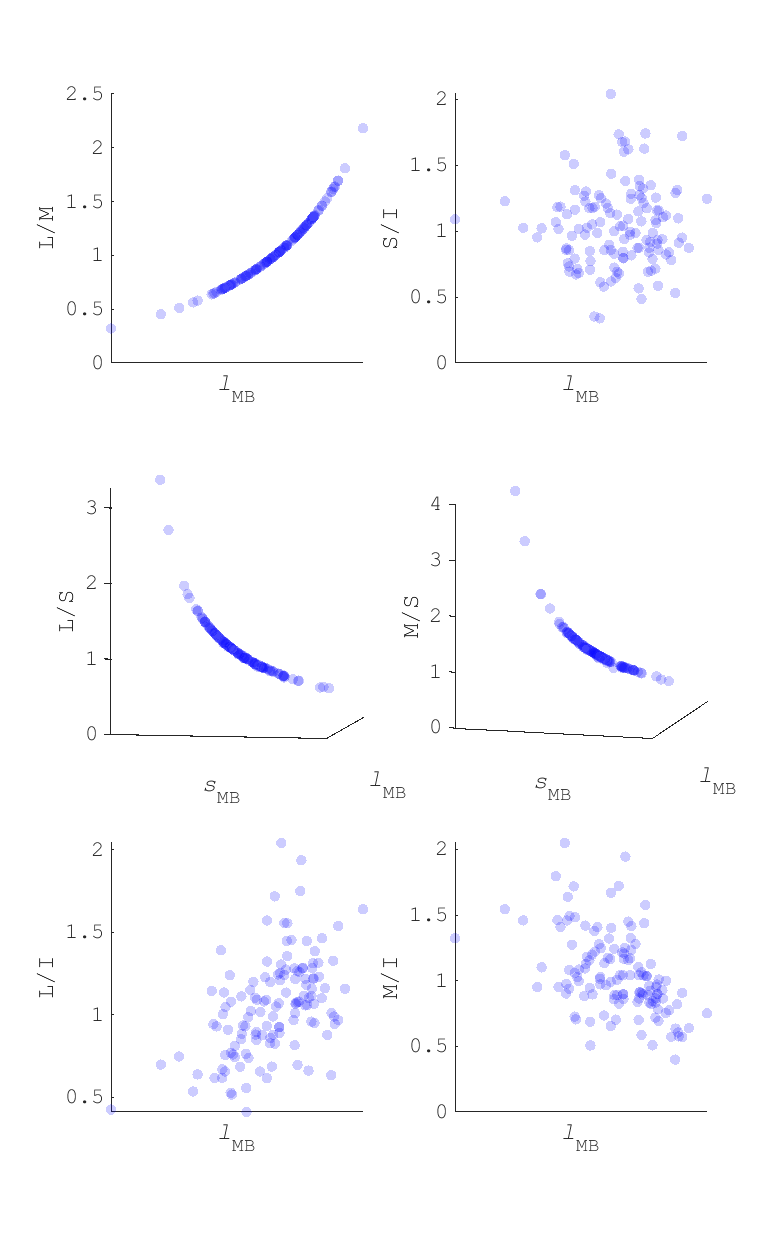
\includegraphics[max width=0.8\textwidth]{figs/comp/predictingChromaticity/allComboSignals_rand.pdf} 
\caption{As per \ref{fig:allComboSignals} but where $[L,M,S,I]$ was replaced by randomly generated values, and the second-level signals were generated from these instead of real values. Blue is used to distinguish this random data from previous real data. Note that different rotations have been applied to some of the subplots to best display the correlations.}
\label{fig:allComboSignals_rand}
\end{figure}

The fact that the relationship between chromaticity and second-level signals degrades for a melanopsin-based second-level signal but not for a cone-based second-level signal, when data is replaced with randomly generated noise, suggests that whilst the relationships in the cone-based cases may arise simply due to the mathematical similarity between the calculation of chromaticity and second-level signals, this is not the case for the melanopsin-based second-level signals. 

Considering that relationships between the melanopsin-based second-level signals and chromaticity do seem to exist (Figure \ref{fig:allComboSignals}), one must conclude that there is a regularity in the data which allows for such a relationship to be revealed.

\bigskip
\noindent
To summarise this section:

\begin{enumerate}
   \item A basic melanopic signal, computed from direct daylight measurements, cannot predict chromaticity (even in a one-dimensional sense, such as predicting \gls{CCT}), other than a crude estimation of whether a measurement is direct sunlight or not. \emph{Figure \ref{fig:level1}}
    \item The same can be said for melanopic values computed for daylight reflected off a surface. \emph{Figure \ref{fig:level1}}
  %  \item A first-level melanopic value is highly correlated with first-level cone signals. \emph{Figure \ref{fig:tristimCorrelation}}
    \item There are relatively strong and simple relationships between hypothetical second-level signals and illuminant chromaticity. \emph{Figure \ref{fig:allComboSignals}}
    \item When considering surfaces, these relationships are maintained, but offset differently for each surface. \emph{Figure \ref{fig:allComboSignals}}
    \item Some of these correlations appear to be nothing more than computational artefacts (\emph{Figure \ref{fig:allComboSignals_rand}}). Notably, the melanopic second-level signals did not seem to be such artefacts.
\end{enumerate}

\section{Transformation to an illuminant-independent space}

Whilst estimating the chromaticity of the illuminant is one way in which colour constancy might be achieved, it is also possible that some transformation might exist which delivers signals into an illuminant-independent space but which doesn't explicitly depend upon an estimate of the chromaticity of the illuminant.

Considering that the absolute melanopic values seemed to offer little predictive benefit (see Figure \ref{fig:level1}) the choice was made to create a normalised melanopic value similar in nature to the MB values. Following Equations \ref{eq:MBTristim} and \ref{eq:MB}, but with a melanopic fundamental, allowed for the creation of what will be termed the $i_{\text{MB}}$ values.

\begin{subequations}
\begin{align}
I_{\text{MB}}&=\sum_{\lambda} \phi(\lambda) \overline{i}(\lambda) \Delta \lambda \\
i_{\text{MB}}&= \frac{I_{\text{MB}}}{L_{\text{MB}}+M_{\text{MB}}} 
\end{align}
\label{eq:iMB}
\end{subequations}

where $\overline{i}(\lambda)$ is the melanopsin fundamental of \citet{lucas_measuring_2014}.


\subsection{A melanopic signal as a third dimension}

In order to understand the relationships between the \gls{MB} chromaticities and the new $i_{\text{MB}}$ values, and to understand what types of corrective computations might be effective, consideration was given to the $i_{\text{MB}}$ signal as a third dimension upon the already two-dimensional \gls{MB} chromaticity space, such as shown in Figure \ref{fig:ZL} (akin to Figure \ref{fig:level1}, but for this new second-level signal). This allowed for the consideration of what properties a signal in this third dimension would need to posses in order to be able to transform the values into a two-dimensional illuminant-independent space.

\begin{figure}[htbp]
 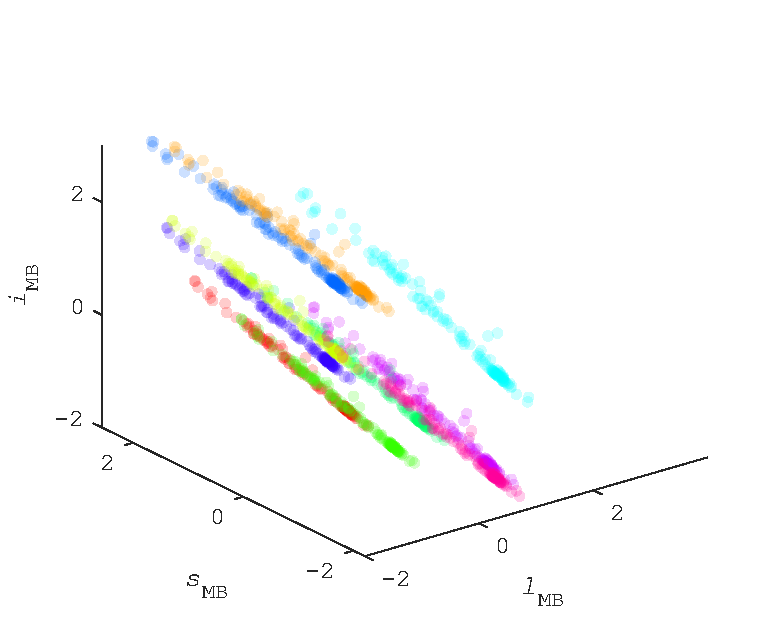
\includegraphics[max width=\textwidth]{figs/comp/thirdDimension/ZL.pdf}
 \caption{X and Y axes are a \gls{MB} chromaticity space, and the Z axis is $i_{\text{MB}}$. Data plotted are same as previous section.}
 \label{fig:ZL}
\end{figure}

It was found that a log transform applied to the $[lsi]_{\text{MB}}$ data made relationships between the various signals more linear, and the data much more normally distributed. A power transformation was also effective in this goal, but a log transform was chosen such that multiplicative transformations could be implemented as additive transformations at later stages. The data were also zero-meaned and normalised for standard deviation so that the signals were on like scales.

A range of speculative transformations were performed, to transform colour signals to illuminant-independent colour signals. A rotational transformation was successful (analogous to changing the perspective as in figure \ref{fig:viewpoint}) and additionally a weighted additive model was found to be rather successful. No satisfactory model was found where a purely multiplicative transformation was applied.

Thinking about a corrective signal as an additional dimension upon a \gls{MB} chromaticity space allows for consideration of requisite or desirable properties that this third signal should imbue upon the three-dimensional cloud of points. I have identified one requisite property, and one desirable property. 

The requisite property for such a signal, as already suggested, is that it should differ from other chromatic signals enough to allow for the point cloud of chromatic points to be significantly \emph{non-planar}. This in turn allows for a projection upon two-dimensional space which has the potential to be illuminant-invariant.

The desirable property is that it should be \emph{roughly monotonic} with respect to other chromatic signals. This allows a one-to-one mapping of colour signals to illuminant-independent colour signals, where a non-monotonic relationship does not necessarily do so. This is not a strict requirement, since the corrective function only needs to be unidirectional, but non-monotonicity would exclude simple transforms (such as linear additive or rotational).

Another key finding at this stage was that there is a perspective upon a three-dimensional point cloud ($[l_{\text{MB}},s_{\text{MB}},i_{\text{MB}}]$) from which points from like objects clustered well, such as in figure \ref{fig:viewpoint}. This property shows that there is at least one transformation such that the points could be projected onto a two-dimensional plane where the illuminant-dependence would be greatly reduced whilst the inter-object chromatic relationships were retained. 

\begin{figure}[htbp] % redo this. Is this log data?
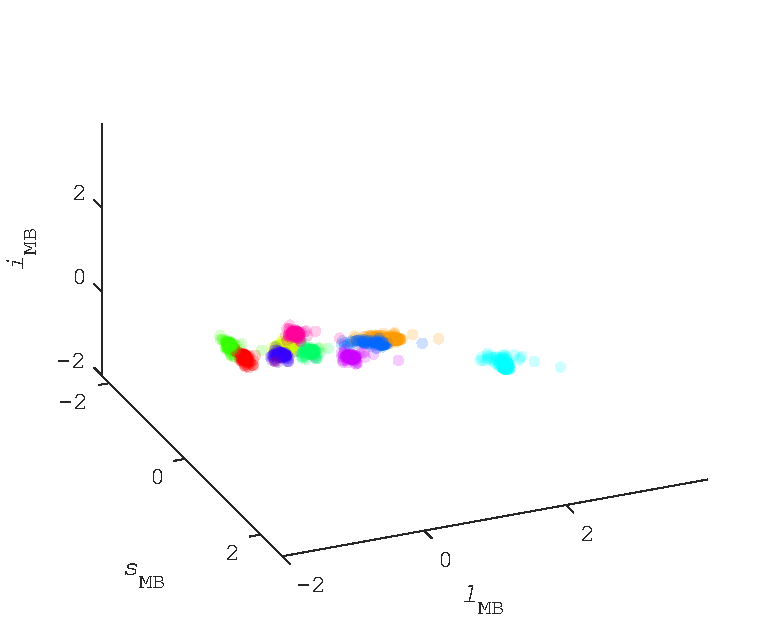
\includegraphics[max width=\textwidth]{figs/comp/thirdDimension/viewpoint.pdf}
 \caption{Figure \ref{fig:ZL} rotated to a perspective where it can be seen that the points project upon a two-dimensional plane in a clustered fashion whilst not degrading to a line within that space.}
 \label{fig:viewpoint}
\end{figure} 

Note that such a perspective would not be possible for a space where the third dimension was a near-duplicate of the first or second, since in this case all points would lie upon a plane. This would be the case in circumstances where a corrective signal too closely resembled the visual signals. The fact that points do not lie on a plane shows that there is some decorrelation between $i_{\text{MB}}$ and both $l_{\text{MB}}$ and $s_{\text{MB}}$. The fact that they do not lie on a plane and instead diverge from this plane in a surface-dependent fashion (as opposed to noisily diverging) suggests that the $i_{\text{MB}}$ may present a means to separate the contributions from illuminant and surface. 

% \subsection{Measuring planarity}

% It also introduced a measure of non-planarity, calculated by performing a principal components analysis on the cloud of points $[l,s,i]_{\text{MB}}$, and looking at how much variance was unaccounted for by the first two principal components. It was found that there were two parts of the spectrum where an effective corrective signal (in terms of non-planarity); firstly at around and just higher than the peak spectral sensitivity of melanopsin, and secondly with a melanopsin shift of about positive 75nm (see `Standard' in Figure \ref{fig:PC3}). It was found that minor changes in parameters used to make these calculations, such as surface set used or observer used, could have moderate effects on the optimal sensitivity for a sensor whose task was to provide a signal for transforming cone signals (see others in Figure \ref{fig:PC3}).

% \begin{figure}[htbp]
%     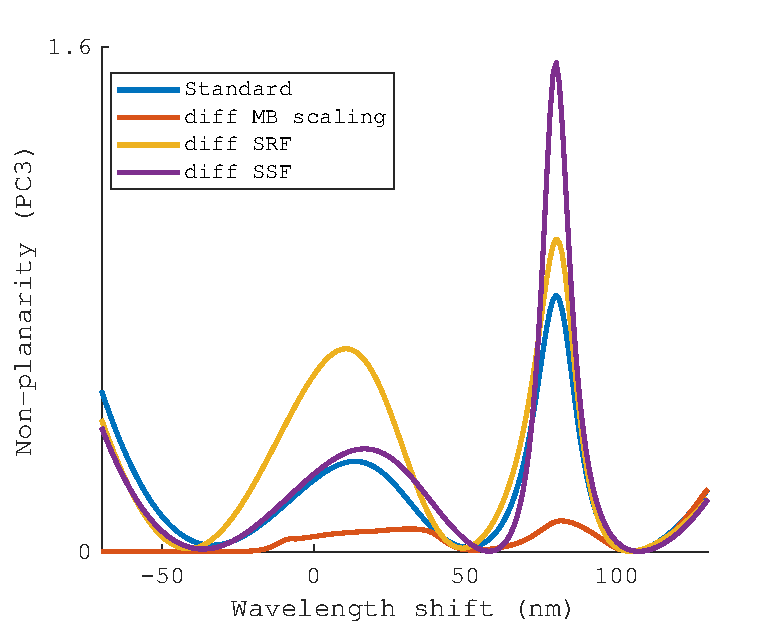
\includegraphics[max width=\textwidth]{figs/comp/melcomp_6/PC3.pdf}
%     \caption{}
%     \label{fig:PC3}
% \end{figure} 



\subsection{Additive/Subtractive model}

It was found that by addition or subtraction of weighted $i_{\text{MB}}$ values, as per equation \ref{eq:correction} conversion to an approximately illuminant-independent space could be performed. An optimisation initially sought optimal weights for the scaling factors with the goal of minimising the overall spread of chromaticities (measured as standard deviation of the entire set). This was later amended to the intra-group spread of chromaticities, measured as standard deviation within each group. This had a relatively minor impact, resulting in coefficient values of $k_{1}$ = 0.57, and $k_{2}$ = -0.94. 

\begin{subequations} \label{eq:correction}
\begin{align}
l_{\text{MB}}* &= l_{\text{MB}} + k_{1}i_{\text{MB}}\\ %these will have changed
s_{\text{MB}}* &= s_{\text{MB}} + k_{2}i_{\text{MB}}
\end{align}
\end{subequations}

where following the optimisation $k_{1}$ = 0.44, and $k_{2}$ = -0.91.

The results of applying Equation \ref{eq:correction} can be seen in figure \ref{fig:corrected}. The effect of different weights can be seen in Figure \ref{fig:minSD}. It can be seen that the points now roughly cluster together by object, with less smearing induced by changes in illuminant (compared to Figure \ref{fig:MB}).

\begin{figure}[htbp]
    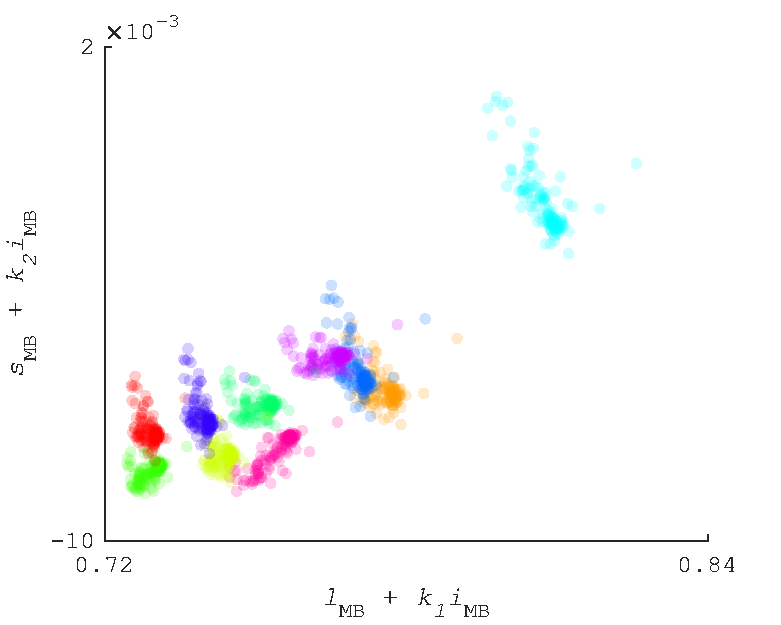
\includegraphics[max width=\textwidth]{figs/comp/transformToIllIndSpace/correctedChromaticities.pdf}
    \caption{\gls{MB} chromaticities for 10 reflectances under 130 daylight illuminants, corrected by the corresponding $i_{\text{MB}}$ value as per Equation \ref{eq:correction}.}
    \label{fig:corrected}
\end{figure} 

\begin{figure}[htbp]
    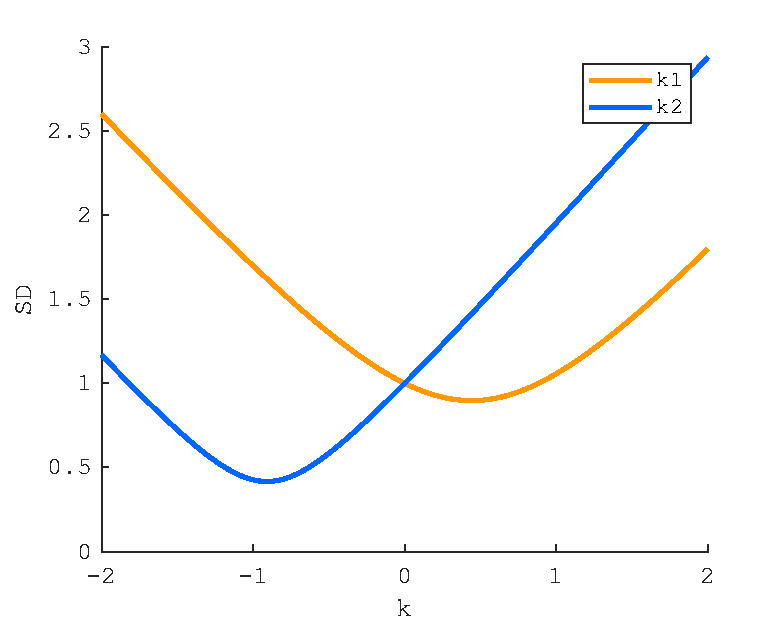
\includegraphics[max width=\textwidth]{figs/comp/transformToIllIndSpace/kvsSD.pdf}
    \caption{The effect on whole-set SD in the relevant dimension ($k_{1}$ applies to $l_{\text{MB}}$ only, and $k_{1}$ to $s_{\text{MB}}$ only) of differently weighted additions/subtractions of the $i_{\text{MB}}$ values. The minima of these functions are taken as the values for $k_{1}$ and $k_{2}$.}
    \label{fig:minSD}
\end{figure} 

It was unclear however whether this advantage would be gained by the addition of any new signal, or whether the melanopsin signal was in any way optimal. With this in mind, the peak spectral sensitivity of the melanopsin function was parameterized, to consider whether shifting it along the wavelength spectrum affected the performance of such a signal. Each new sensitivity function was allowed the benefit of its own weighting optimisation, allowing different scaling factor weights. The results of this computation can be seen in figure \ref{fig:opt}. 

\begin{figure}[htbp]
    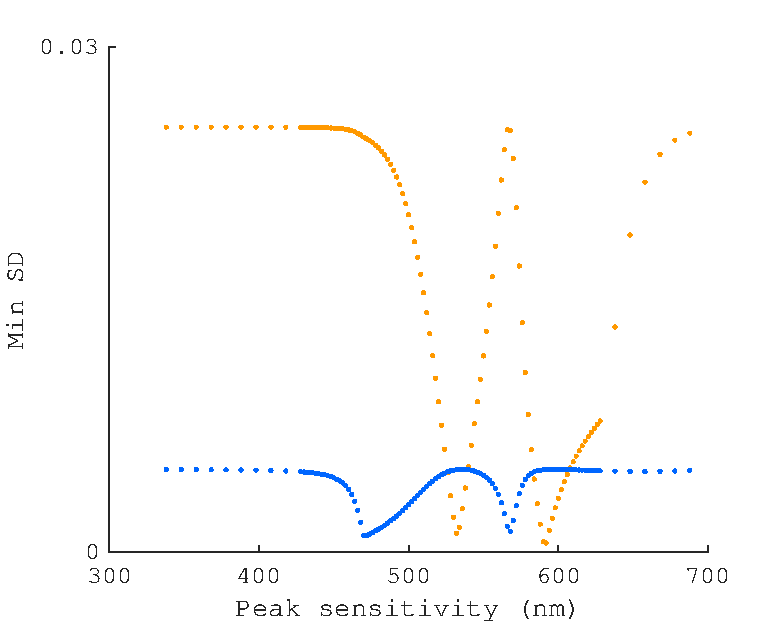
\includegraphics[max width=\textwidth]{figs/comp/transformToIllIndSpace/offsetrange1.pdf}
    \caption{The results of an optimization where the spectral sensitivity of the nominal melanopsin fundamental was shifted along the spectrum.}
    \label{fig:opt}
\end{figure} 

The standard deviation minima for $l_{\text{MB}}$* occur at 532nm and 590nm, and for $s_{\text{MB}}$* at 444nm and 568nm. This would suggest that the optimal spectral sensitivity for a receptor employed to correct the signals from the various cones would be at these points in the spectrum. However, if we plot the transformed chromaticities computed using hypothetical signals at these wavelengths, we see that the results are not an obvious improvement. In Figure \ref{fig:590} the results of using a nominal melanopic signal with a peak spectral sensitivity of 590nm are shown. Group SD is low, but different surfaces are not particularly well distinguished from each other. We witness good colour constancy, at the expense of chromatic discrimination\footnote{At my poster at VSS David Brainard referred to this as the `Ford Model of Colour Constancy' - you can have any colour, so long as it's black.}. This is obviously not ideal.

\begin{figure}[htbp]
    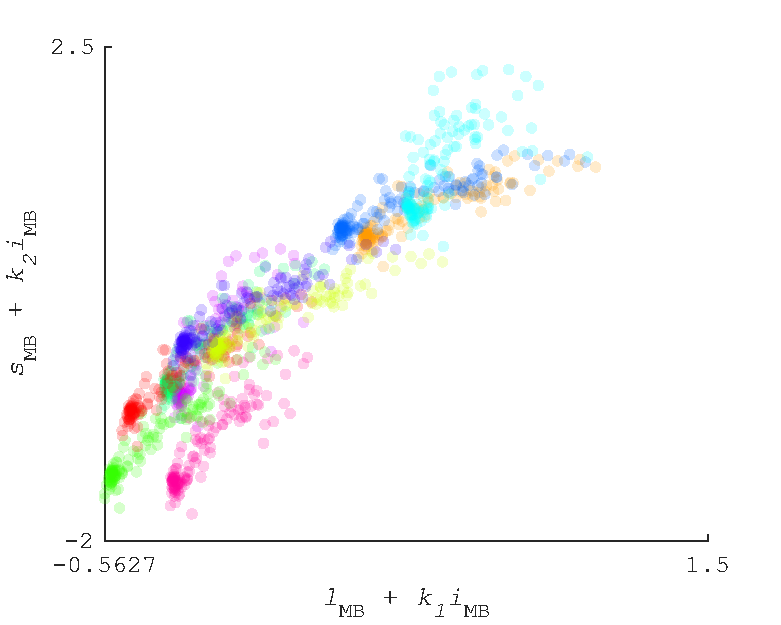
\includegraphics[max width=\textwidth]{figs/comp/transformToIllIndSpace/correctedChromaticities_range590.pdf}
    \caption{The `corrected' values using a nominal melanopic signal with a peak spectral sensitivity of 590nm.}
    \label{fig:590}
\end{figure} 

This result made it very clear that more thought was required regarding how `success' was calculated.

The actual desired behaviour would be to minimise internal variance for each reflectance group (rather than the whole set), whilst maintaining at least some distinction between inter-reflectance groups. There are various ways to implement this, which will be covered in the following sections. %

\bigskip
\noindent
To summarise this section:
\begin{enumerate}
    \item Following earlier findings that a second-level signal seemed more likely to show a relationship to chromaticity, and be likely to sample the \gls{PC2} values of daylight, hypothetical $i_{\text{MB}}$ values were computed.
    \item Various transformations were trialled: additive/subtractive, rotational and multiplicative. The first two showed promise (and seemed to be roughly interchangeable), whereas no adequate multiplicative transformation was found.
    \item One requisite and one desirable property for a hypothetical third signal were identified: decorrelation (leading to non-planarity) and monotonicity. 
    \item A perspective upon the three-dimensional $[lsi]_{\text{MB}}$ space was found where points diverged from a plane in a surface-dependent fashion. \emph{Figure \ref{fig:viewpoint}}
    \item A basic additive/subtractive algorithm was applied, which seemed to reduce the spread of chromaticities in a meaningful fashion. \emph{Figure \ref{fig:corrected}} 
    \item It was found that when the melanopic value was replaced by signals generated from different spectral sensitivities, some hypothetical signals appeared to be more successful than a melanopic value. These signals performed very well by the metric of whole-set standard deviation, but in practice would make very poor corrective signals due to the reduced discriminability between surfaces. \emph{Figure \ref{fig:590}}
\end{enumerate}


\section{Assessment of colour constancy algorithms}

The basic mechanism of an additive/subtractive model of melanopic colour constancy seems worthy of further scrutiny. However, we have seen that care is required in defining what is considered successful performance for a colour constancy algorithm. Broadly speaking, we would like our algorithm to be judged on its ability to allow for \emph{recognition} (reliably remapping points from a specific surface to a specific point in appearance space) and \emph{discrimination} (creating distinct representations of different surfaces)\footnote{The ideal colour constancy algorithm would distinguish between all spectrally distinct surfaces, no matter how minor their distinctions. However, here we are more interested in uncovering a mechanism which may be used by the human visual system, and so it seems sensible to limit the requirement to separation of surfaces which would generally be seen as chromatically distinct.}.

Different schools of thought within colour constancy research have used different methods for assessing proposed algorithms, mirroring subtle differences in their respective conceptual goals. Three subtle variants can be described via representative research questions:

\begin{itemize}
\item{How do humans achieve colour constancy?}
\item{How do we predict what humans perceive?}
\item{How can we colour correct digital photos to emulate the original appearance of the scene to the photographer?}
\end{itemize}

The first group have tended to assess their proposed solutions in the context of biological and physical plausibility. Where solutions in this group rely upon some regularity in the environment, discussions gravitate to the value, ubiquity, and veracity/validity of this regularity (see Hurlbert's table \cite[p.~295]{hurlbert_computational_1998} which sorts a range of colour constancy algorithms by the assumptions that they rely upon). Alternatively, studies can remove the cue or cues under investigation from a controlled visual scene and in some way measure the impact upon an observer's state of chromatic adaptation \cite{kraft_mechanisms_1999}. I am not aware of a standard measure for quantifying the ability or biological plausibility of a particular proposed algorithm.

The second group have made considerable progress in the development of the \Glspl{CAT} which are used within \Glspl{CAM}, through the collection of corresponding colour datasets (pairs of colorimetric values where the the first member of each pair under a first illuminant matches in appearance the second under a second illuminant). Models are then fitted to these datasets such that the appearance of an arbitrary colour under the one illuminant could be predicted under the other, and vice versa. The effectiveness of a model is quantified by considering how well the model fits data that was independently collected \cite{cie_cie_2004-1}.

The third group focuses on estimating the tristimulus values or colorimetry of an unknown illuminant from the pixels of a digital photographic image. There is obvious crossover between this group and the previous groups, for two reasons.
Firstly, the human visual system could compute relatively meaningful estimates of surface reflectance properties if the illumination spectra could be estimated with moderate accuracy \cite{maloney_computational_1984}. Secondly, where the goal is to output an image which appears as it would to a human observer, there is implicitly a goal to understand how an observer might be performing this computation. This group traditionally quantifies success of algorithms by how well they can compute an illuminant estimate in terms of its RGB values in a camera-specific colour space.

There is no clear fit between existing models of assessment and the specific goals of the algorithm under assessment. The most natural fit is within the first group, since the key interest is whether a melanopsin-based signal provides a valuable tool to a biological system in solving an ecological problem (and thus whether it might exist in real biological systems). However, it is unclear at this stage what is the mechanism by which such a system may operate, and so the discussion of what assumptions such a mechanism may rely on seem overly abstract.

Of clearer applicability is the work of Barnard et al. \cite{barnard_comparison_2002} (later used by \citet{hordley_reevaluation_2006} and \citet{gijsenij_computational_2011}). They propose a method whereby spectral measurements of illuminants and surfaces are used to create `synthesized' data, representing each surface under each illuminant, which can be used as an input to a colour constancy algorithm. Since the ground truth is known here, the results can be quantitively assessed. 

There are some amendments to their process which are required if we are to use it here. Firstly, the data used in their experiments comprises natural and non-natural surface reflectances and illuminants, which is suitable for their purposes of assessing algorithms designed for digital cameras, but is unsuitable here for assessing an algorithm to understand its ability in a natural environment (the environment which would have influenced the natural evolution of biological systems). Therefore, the reflectance and illuminant data will need to be limited to naturally occuring data. Secondly, their performance metrics again relate to their problem rather than ours: they consider only the accuracy of the estimated white point, and whilst this may be useful to a biological system, the grander goal is a conversion of chromaticities to an illuminant-independent surface appearance space. An illuminant estimate is one way to reach this goal, but it is not fundamentally necessary, and the accuracy of this value does not necessarily provide a good measure of effectiveness of the whole system.

One performance metric which more closely matches the goals of this study is that provided by Forsyth \cite[p.~19]{forsyth_novel_1990}, who suggests ``the median Euclidean distance of the outputs from the average (over the different lights) output, for each [colour] chip. This median is then normalised by the Euclidean magnitude of the outputs.'' This value provides an insight into the nature of the clustering of points following a transform, which can be considered as loosely related to our fundamental goal of allowing for recognition (a point being mapped to roughly the point it should be). However, no regard is given to our second fundamental goal of discrimination. Indeed, an algorithm which outputs two clusters of points which lay directly atop each other, even if these clusters represented vastly different objects, would be rated as successful, if these clusters were particularly tightly clustered.

% ---------------------------------- %
\subsection{K-means clustering as an assessment tool}

Whilst the clustering metric of Forsyth is a step in the right direction, it doesn't quantify disriminability, and there is no clear way in which it could be amended to do so. Further, it would be preferable to consider these two characteristics in unison since they are valuable only in relation to each other: we could allow for loose clustering if the cluster centres were distant, but require tight clusters if they were close. 

To address this shortcoming I propose the following: that the output of an algorithm (where the input is a batch of synthetic data such as in the method of \citet{barnard_comparison_2002}) should be subjected to a k-means clustering (this is easy where synthesised data is used and $k$ is known) and this output in turn should be marked against the known groupings of the original input data. This marking would reveal how well the algorithm had remapped points into clusters relating to their original grouping, and how separable the clusters are. A suitable number of repetitions of the k-means clustering is advisable, to avoid local minima. 

% A more extensive framework of testing a melanopic correction against other colour constancy algorithms was introduced, following the framework of \citet{barnard_comparison_2002} (later used by \citet{hordley_reevaluation_2006} and \citet{gijsenij_computational_2011}) A \gls{GW}, a \gls{BiW}, and a \gls{DN} algorithm were used as benchmarks.

To test/demonstrate such a procedure, let us consider the plots from Figure \ref{fig:corrected} and \ref{fig:590}. Whilst the simple measure of whole-set standard deviation reports the latter as the more successful output, the k-means-mark for these outputs is 0.8915 and 0.5662 respectively, which tallies with our intuition of which instance of the algorithm has performed better. The K-means selections for each are visualised in Figures \ref{fig:KM1} and \ref{fig:KM2}.

Before the k-means clustering algorithm was applied, data were again zero-meaned (no effect on algorithm, only neatens later presentation) and normalised by standard deviation (medium/large effect on algorithm, resulting in equal weights given to variance in either dimension of \gls{MB} space).

\begin{figure}[htbp]
 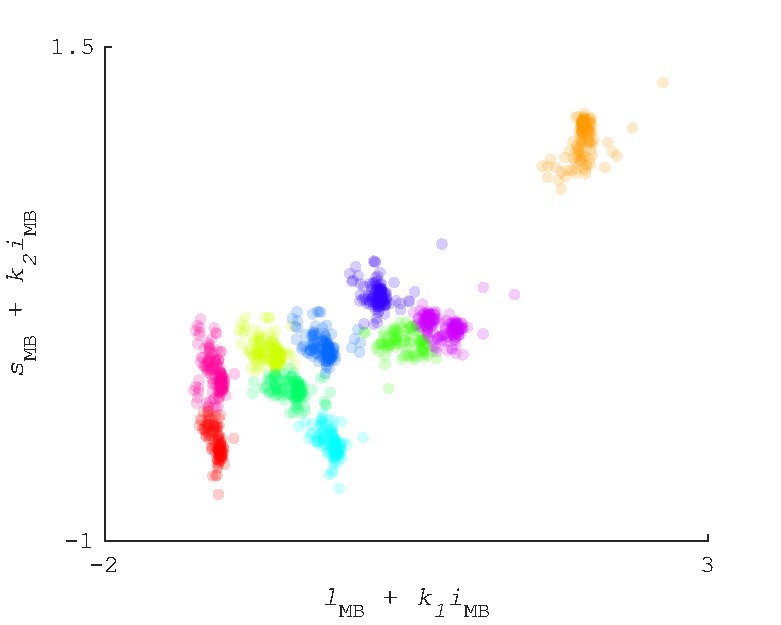
\includegraphics[max width=0.8\textwidth]{figs/comp/KMeansMarkDemo/1.pdf}
 \caption{The data of Figure \ref{fig:corrected}, plotted with colours indicating the groupings chosen by a k-means clustering procedure. Note that the colours do not relate to appearance of surfaces, they are only to indicate groupings. Note also that these colours do not correspond to colours used in the previous figure; the k-means-mark algorithm is not interested in the absolute labelling of groups, rather whether all members from group X have been sorted into group Y etc.)}
 \label{fig:KM1}
\end{figure} 

\begin{figure}[htbp]
 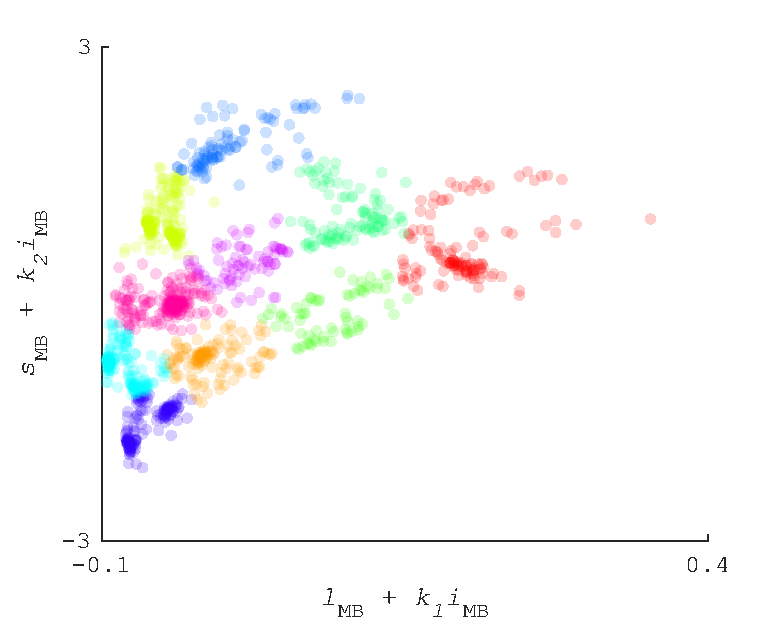
\includegraphics[max width=0.8\textwidth]{figs/comp/KMeansMarkDemo/2.pdf}
 \caption{The data of Figure \ref{fig:590}, plotted with colours indicating the groupings chosen by a k-means clustering procedure.}
 \label{fig:KM2}
\end{figure} 

% ------------------------- %

\subsection{A comparison of four algorithms}

The simple melanopic algorithm (additive/subtractive) was compared with 3 other algorithms: a \gls{GW} algorithm, a \gls{BiW} algorithm and a \gls{DN} algorithm (a baseline condition where no correction was applied). The structure of \citet{barnard_comparison_2002} was employed, but with the modifications suggested above. %This is shown as a flow diagram in Figure \ref{fig:flow}. 

% \begin{fullpagefigure}
% \figpdf[pages=-,rotate=90, offset=75 -75]{figs/comp/flow.png}
% \caption{A flow chart representation of the assessment process.}
% \label{fig:flow}
% \end{fullpagefigure}

The results of the four algorithms are shown in Figure \ref{fig:output100}. It can be seen that the \gls{GW} algorithm performs particularly well under this test condition, separating the different surfaces into very tightly clustered and very distant groups. The \gls{BiW} algorithm appears to choose one of two surfaces as the brightest, which splits each surface group into two groups. If it were able to pick a single reference point it appears as though it would be similarly successful. The melanopsin-based correction performs moderately well; as shown before it improves greatly upon the \gls{DN} condition, but the groups are not particularly tightly clustered and there is a moderate amount of overlap between the groups.

This visual analysis is mirrored by the k-means-marks computed for each output. They were: \gls{DN}: 0.5869, \gls{GW}: 0.9631, \gls{BiW}: 0.5308, mel-based: 0.9346.\footnote{It should be noted that due to the random nature of initial seeding in k-means clustering, these values are expected the vary slightly depending on initial state of the random number generator.}

\begin{figure}[htbp]
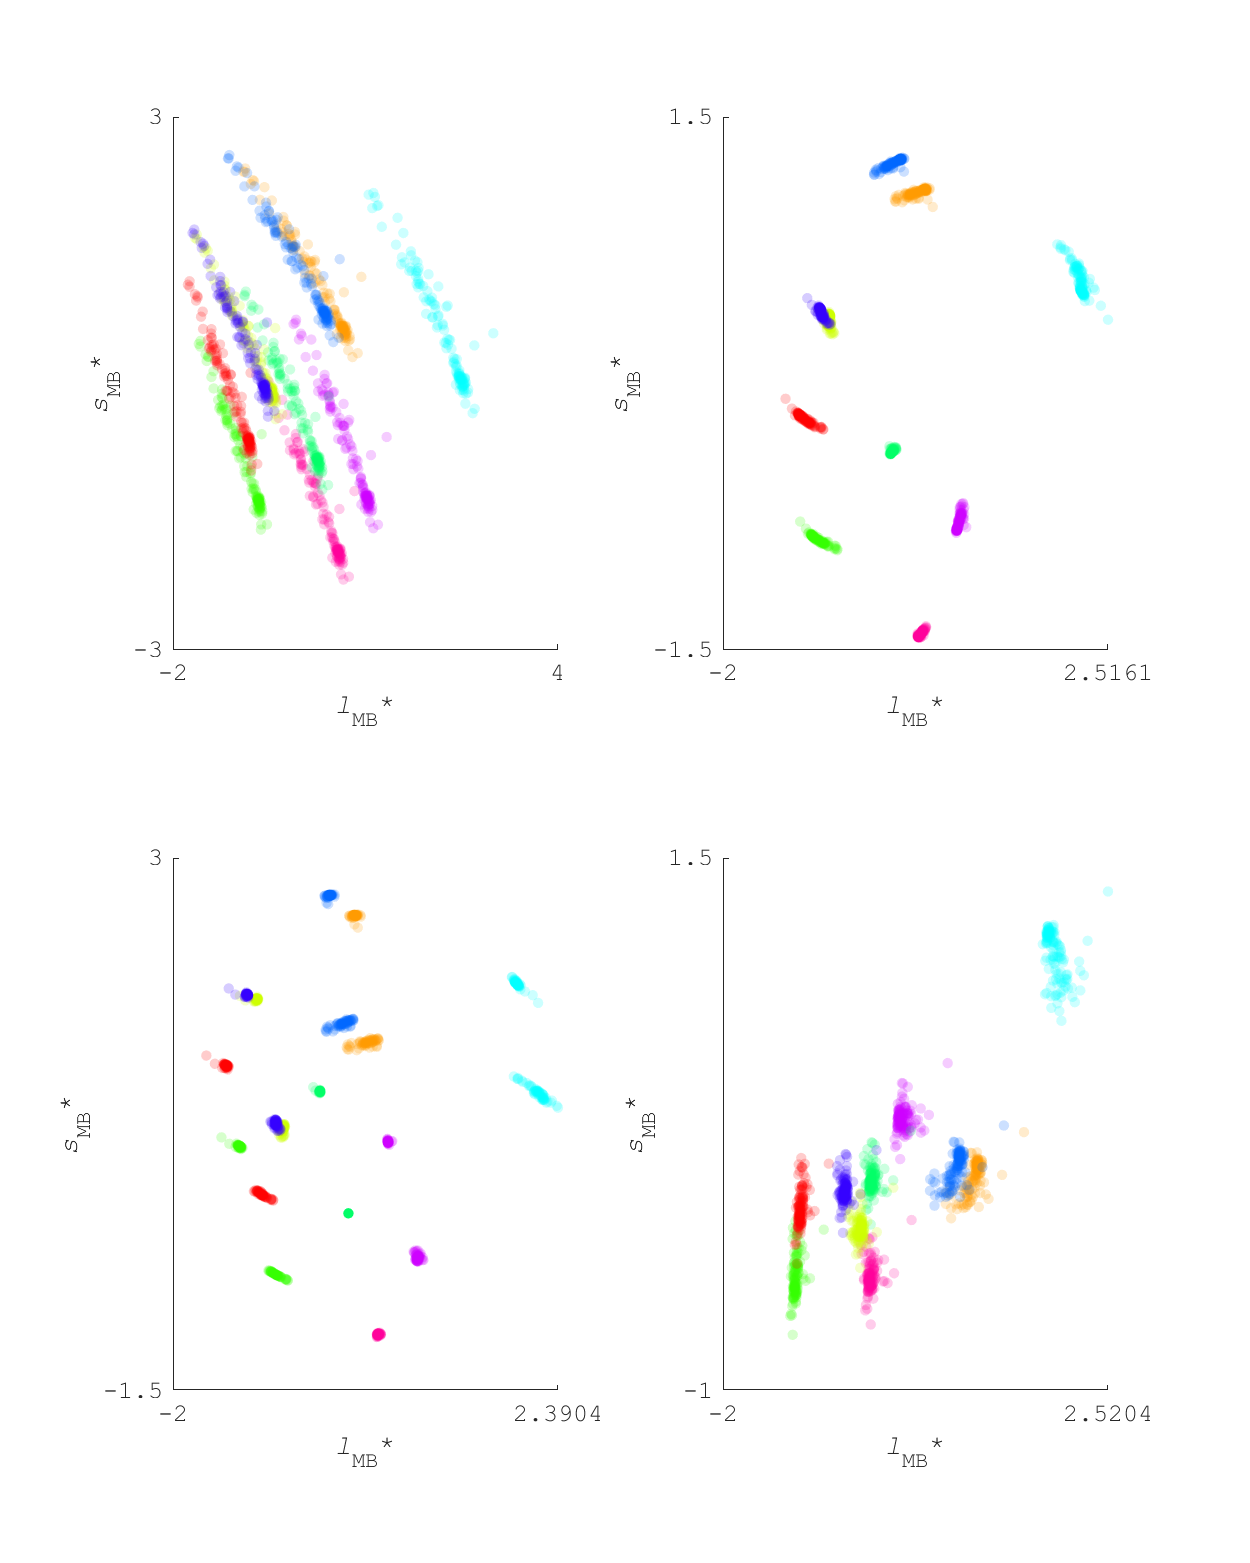
\includegraphics[max width=1.2\textwidth, center]{figs/comp/comparisonFourAlgos/output100.pdf}
 \caption{The output of the four algorithms; top left: \gls{DN}, top right: \gls{GW}, bottom left: \gls{BiW}, bottom right: melanopsin-based correction, as per Equation \ref{eq:correction}. Colours denote different surface groups.}
 \label{fig:output100}
\end{figure} 

\begin{figure}[htbp] % From the next section but I really want these to be next to each other
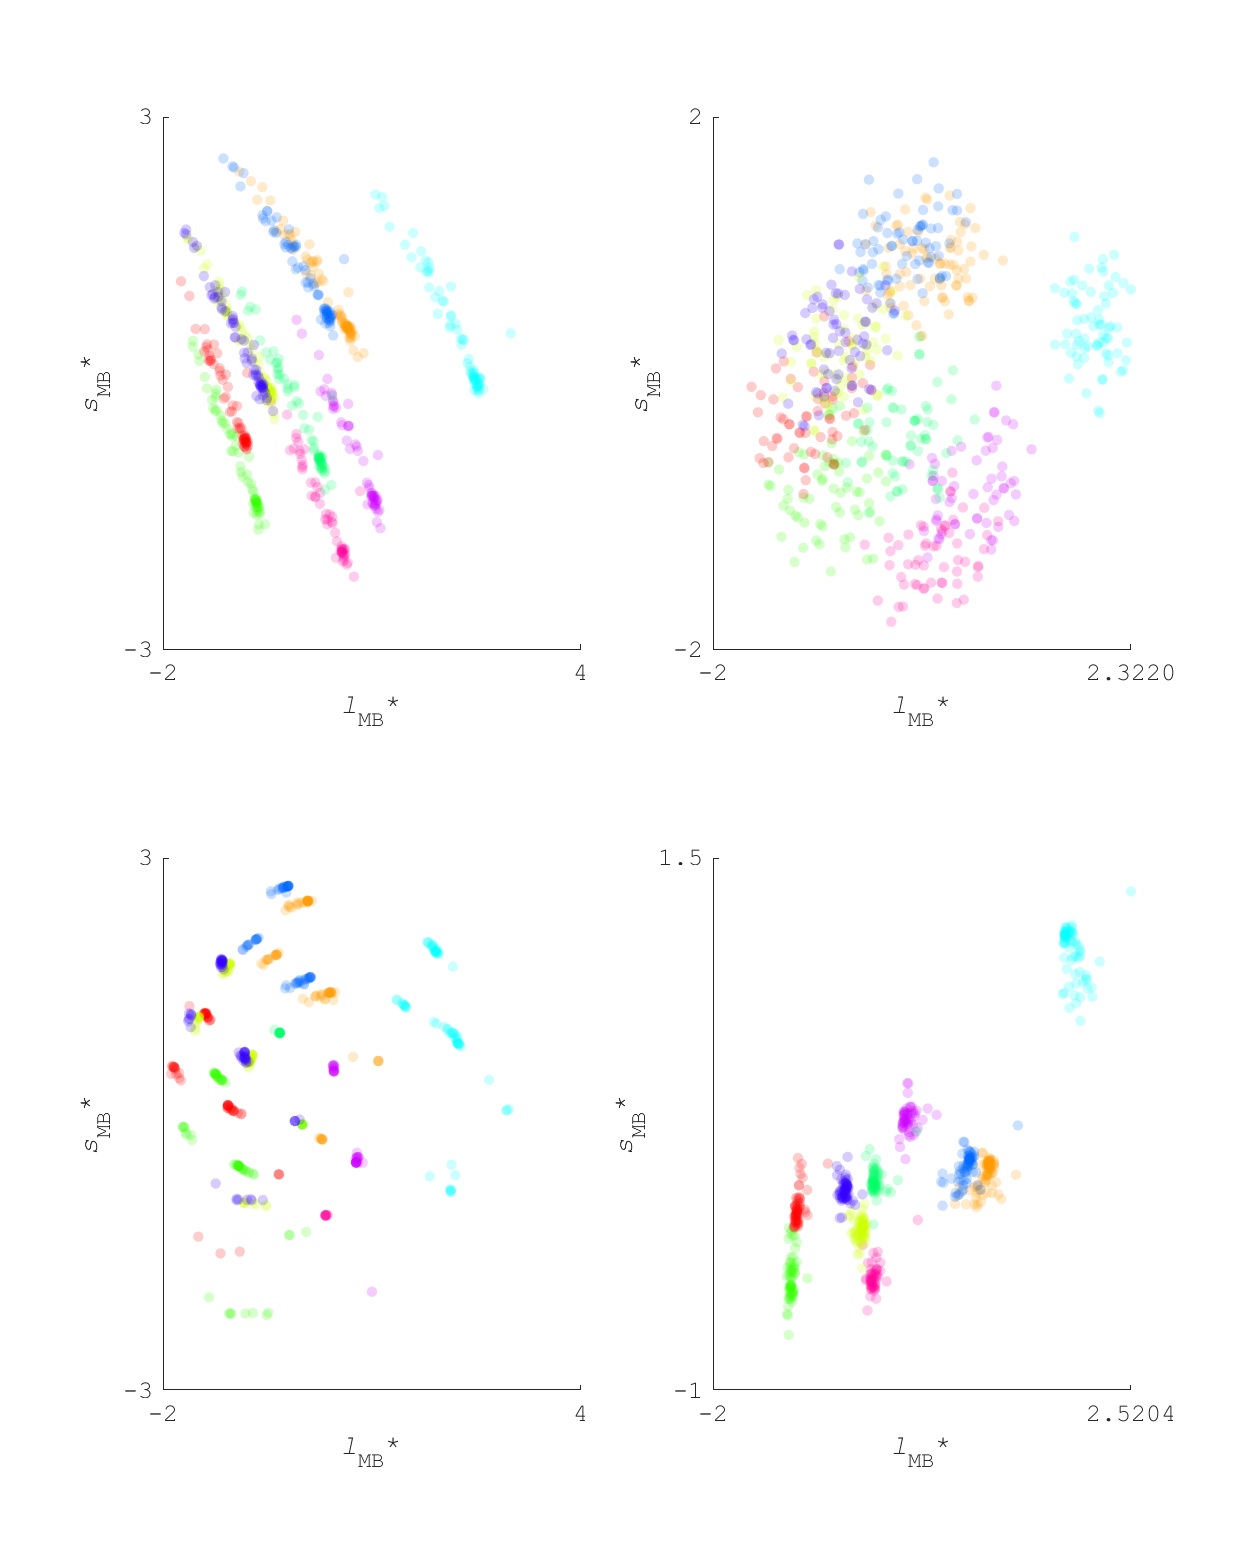
\includegraphics[max width=1.2\textwidth,center]{figs/comp/comparisonFourAlgos/output50.pdf}
 \caption{As per Figure \ref{fig:output100} but where only 50\% of the surfaces are present under each illuminant.}
 \label{fig:output50}
\end{figure} 

% ---------------------------------- %

\subsection{A more naturalistic test case}

In terms of real-world validity, this test condition represents a rather unusual situation: a set of 10 surfaces is represented under each illuminant, with each surface always being present, in the same proportion (relative to other surfaces) each time. Under these conditions, we should expect \gls{GW} and \gls{BiW} to flourish. In more realistic conditions however (where the scene was less stable), we might expect them to suffer.

When we randomly remove 50\% of the surfaces under each illuminant, the resulting k-means-marks are: \gls{DN}: 0.5989, \gls{GW}: 0.6967, \gls{BiW}: 0.5916, mel-based: 0.9447. It can be seen that \gls{GW} has fallen dramatically whilst the others have remained roughly stable. 

A visualisation of the results at under this condition is shown in Figure \ref{fig:output50}. It can be seen that the neat clusters that \gls{GW} showed in Figure \ref{fig:output100} have degenerated into broad clouds. This can be explained by the cue that \gls{GW} uses becoming noisier; when viewing unknown surfaces drawn from a normally distributed set of surfaces (in terms of chromatic bias), the fewer surfaces that are visible, the lower the likeliood that the mean chromaticity of the surfaces represents the chromaticity of the illuminant. 

Parameterising the percentage of surfaces shows that this general trend continues at other percentages. Outcomes at percentages from 20\% to 100\% in 10\% intervals are shown in Figure \ref{fig:outputRange}.

\begin{figure}[htbp]
 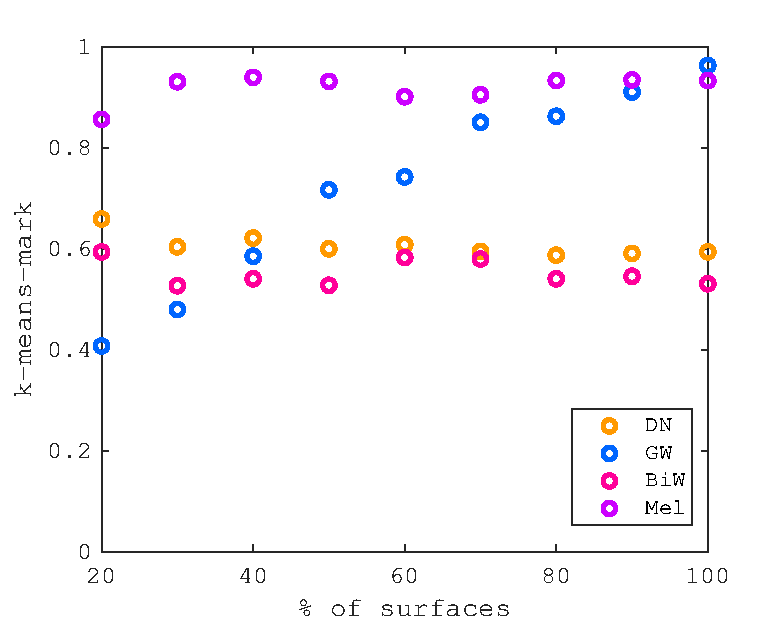
\includegraphics[max width=\textwidth]{figs/comp/comparisonFourAlgos/outputRange.pdf}
 \caption{The performance of the various algorithms as a function of the available surfaces (100\% = 10).}
 \label{fig:outputRange}
\end{figure} 

Increasing the number of surfaces has little effect on the overall trend. A trial performed with 32 surfaces from the \citet{vrhel_measurement_1994} dataset (selected such that they were `natural' and above a minimum threshold chromaticity difference (calculated under a single daylight measurement) showed a slight overall decrease in the performance of the melanopsin-based correction, but it still outperformed all other algorithms below 80\% surface inclusion. Interestingly, the \gls{BiW} algorithm performed much better than it had in previous trials, presumably within this subset of the data the brightest surface was a more reliable cue than in the previous set. A summary for this test is shown in Figure \ref{fig:outputRangeMore}

\begin{figure}[htbp]
 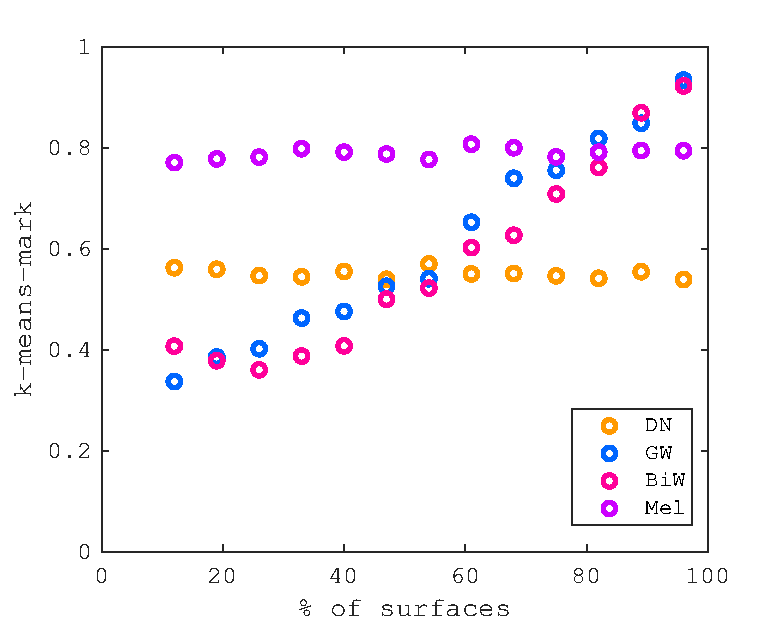
\includegraphics[max width=\textwidth]{figs/comp/comparisonFourAlgos/outputRangeMore.pdf}
 \caption{As per Figure \ref{fig:outputRange} but with an extended set of 32 \glspl{SRF}.}
 \label{fig:outputRangeMore}
\end{figure} 

\bigskip
\noindent
To summarise this section:
\begin{enumerate}
    \item The analysis of colour constancy algorithms by previous research groups was considered, noting their distinct aims within the colour constancy field.
    \begin{enumerate}
        \item The framework of \citet{barnard_comparison_2002} was employed: synthetic stimuli were produced.
        \item The clustering method of \citet{forsyth_novel_1990} was considered, but found unsuitable.
        \item A modification whereby the algorithm output was subjected to a k-means clustering analysis, and the computed clusters were compared to ground-truth clusters, was proposed.
    \end{enumerate}
    \item Four colour constancy algorithms were tested.
    \begin{enumerate}
        \item Under the baseline conditions, whereby each surface was presented once under each illuminant, the \gls{GW} algorithm performed best, followed closely by the melanopsin-based transform.
        \item Under more naturalistic conditions, where a new random subset of 50\% of the reflectances was shown under each illuminant, the performance of the \gls{GW} algorithm dropped drastically.
        \item This trend was shown to hold at other percentages of surfaces included and for larger surface sets.
    \end{enumerate}
\end{enumerate}

% ---------------------------------- %

\section{Optimality of the melanopsin spectral sensitivity}


Now that we have a seemingly robust method for quantifying the performance of an algorithm, we are better placed to consider whether the \gls{SSF} of melanopsin is in any way `optimal' for this task, or whether any performance stems simply from allowing this particular algorithm to have access to a greater amount of information through additional sampling of the scene.

Re-running these computations but shifting the spectral sensitivity of the nominal melanopsin \gls{SSF} to lower and higher wavelengths, gives Figure \ref{fig:optimality}. At each wavelength a new optimal pair of $k$ values (Equation \ref{eq:correction}) was computed. The computations were re-run 10 times, and the minimum, mean and maximum taken for each point. This variability exists only because of the random seeding required for the k-means clustering algorithm. Within the standard script there are 20 repeats of each k-means-mark test, and presumably if this figure was raised the variability visible in Figure \ref{fig:optimality} would disappear.

\begin{figure}[htbp]
 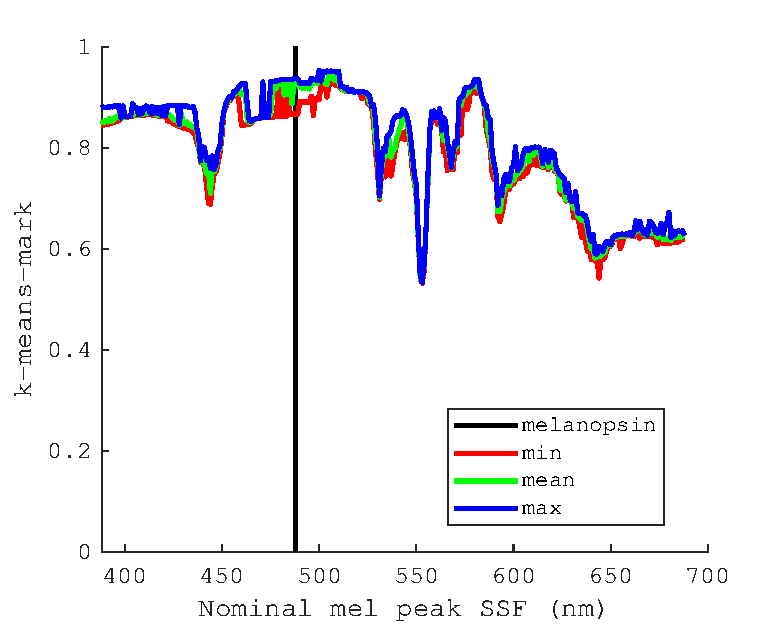
\includegraphics[max width=\textwidth]{figs/comp/optimality_caller/optimality.pdf}
 \caption{The results of varying the peak wavelength of the nominal melanopsin spectral sensitivity function.}
 \label{fig:optimality}
\end{figure} 

It can be seen that the baseline spectral sensitivity of melanopsin (peak at 488nm) is in the best area of the spectrum for a signal which is to be used for correction in this fashion (peaking at around 510nm). There is an additional peak at around 582nm. It may be coincidental, but it seems worth noting that the spectral sensitivity of the bistable form of melanopsin would be at 587nm \citep{mure_melanopsin_2009}.


% -------------%

\section{Why is this possible?}


At this stage the underlying reason for the relative success of these transforms was considered. One potential lead is a curious regularity at the shorter wavelengths of the reflectance spectrum of many natural objects. In figure \ref{fig:plateau} it can be seen that there is a plateau in the relative spectral reflectances of some natural objects (a subset of the \citet{vrhel_measurement_1994} reflectances) between approximately 430nm and 480nm, with relatively small deviations in the range 400nm to 500nm. Another way to visualise this is to calculate the correlation between points on the reflectance function. Such a calculation was performed initially on a combined set of scenes 1-4 of the
\citet{nascimento_statistics_2002}\footnote{Data: \url{https://personalpages.manchester.ac.uk/staff/d.h.foster/Hyperspectral_images_of_natural_scenes_02.html}} hyperspectral reflectance data and
scenes 1-5 of the 
\citet{foster_frequency_2006}\footnote{Data: \url{https://personalpages.manchester.ac.uk/staff/d.h.foster/Hyperspectral_images_of_natural_scenes_04.html}}
hyperspectral reflectance data, and then on three other datasets. See Figures \ref{fig:foster} and \ref{fig:others} respectively.

\begin{figure}[htbp] % update this to look better and include the specific data used elsewhere in this section
 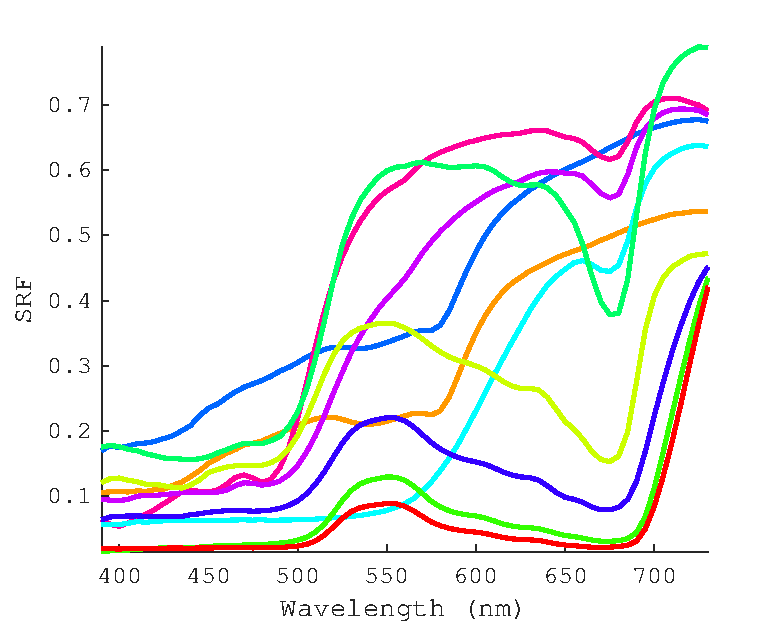
\includegraphics[max width=\textwidth]{figs/comp/plateau.pdf}
 \caption{The spectral reflectance functions of a subset of the \citet{vrhel_measurement_1994} reflectances (solid lines), normalised at the peak of s-cone sensitivity (CIE 2006 10$^{\circ}$), with the spectral sensitivity of s-cones and melanopsin \citep{lucas_measuring_2014} overlaid (dot-dashed lines).}
 \label{fig:plateau}
\end{figure} 

\begin{figure}[htbp]
 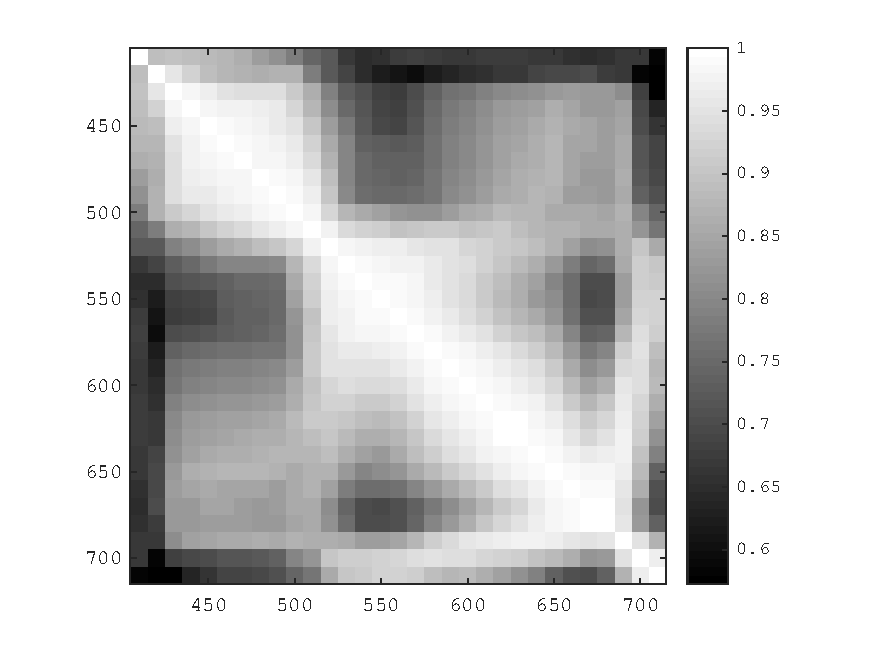
\includegraphics[max width=\textwidth]{figs/comp/nat_cor/foster.pdf}
 \caption{Visualisation of the average correlation matrix for the scenes 1-4 of \citet{nascimento_statistics_2002} and 1-5 of \citet{foster_frequency_2006}. Note the lighter square region in the top left, indicating an area of increased correlation across different wavelength samplings, and another square region (though with a faded lower-right corner) in the centre. The dark frame to this figure is likely due to increased measurement noise at these extremes. The figure is symmetric about the diagonal axis.}
 \label{fig:foster}
\end{figure} %get rid of dotted line on colorbar

\begin{figure}[htbp]
 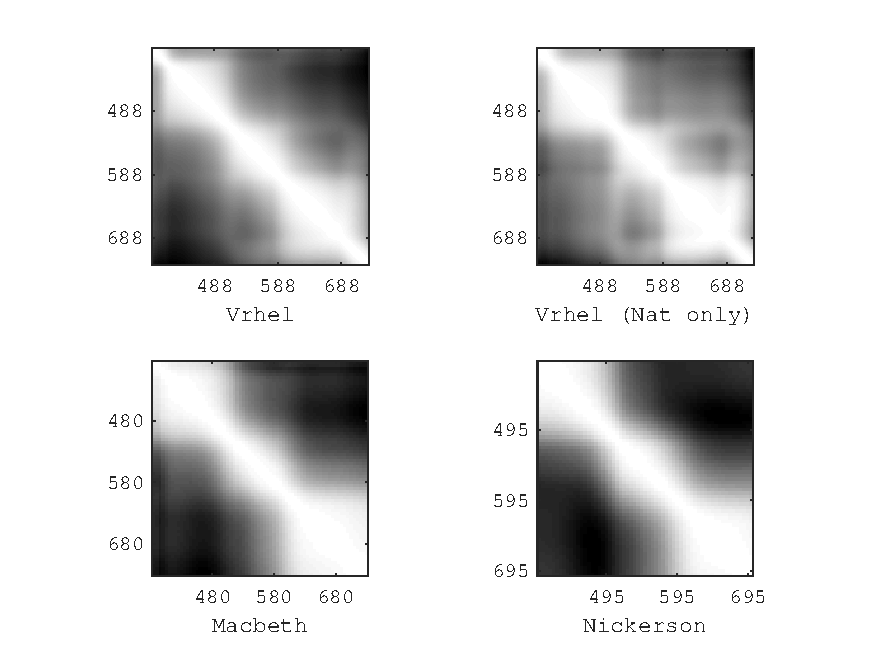
\includegraphics[max width=\textwidth]{figs/comp/nat_cor/others.pdf}
 \caption{As for \ref{fig:foster} but for 3 different sets of data, and one subset. `Vrhel' refers to the object reflectances of \citet{vrhel_measurement_1994} data and `Vrhel (nat only)' refers to a subset of the previous but only using data for surfaces which were deemed `natural'. `Macbeth' refers to measurements of a Macbeth Color Checker. `Nickerson' refers to a set of measurements of Munsell papers (presumably the \citet{kelly_tristimulus_1943} data). Note that whilst we have a selection of real surfaces, natural surfaces, and printed papers, all plots show similar trends, with three areas of correlation, at low, medium and high wavelengths. The low wavelength square seems to match that in Figure \ref{fig:foster} well, but the other two areas are only really distinguishable in this second set of figures. All data obtained via \gls{PTB} (`sur\_vrhel', `sur\_macbeth', `sur\_nickerson').}
 \label{fig:others}
\end{figure} 

An interesting advantage could be made of this regularity. Assume a simpler situation where there were two points on the spectrum of the reflectance functions of a set of natural objects which were always the same as each other (perfect correlation). Sensors of appropriately narrow spectral sensitivity, placed at these two points on the spectrum would always register corresponding signals. Considering that the second principal component of daylight variability is a broad skew, any difference in the signals from two such receptors could be used fairly reliably to sense the contribution of this second component in any single condition. 

%Summary: The underlying reason for the relative success of the investigated transforms was considered. A plateau at shorter wavelengths of natural object reflectances was noted, and it was speculated that this could be taken advantage of.

\clearpage

% --------------------------------------%

\section{Conclusions}

In this exploratory computational study, the goal was to understand whether a signal from a melanopsin-expressing cell might be useful colour constancy.

The first question was whether a melanopic signal could be used as a cue to the illuminant. Following the investigation, this seems like rather a naive question, but it is worth recalling that this (or something close) is the underlying assumption in our previous studies. It is now clear that a raw melanopic signal (not normalised in any fashion) can only provide a very crude cue to the chromaticity of the illuminant: if it is above a certain threshold then it can be assumed that the illuminant on the scene is direct sunlight, which has a relatively reliable chromaticity. This signal notably is also strongly correlated with the other retinal signals, and therefore provides no clear additional value.

One line of enquiry which may be valuable to pursue, and which may provide a reprise for a raw melanopic signal, would be to consider the problem through the lens of a Maloney-Wandell-type linear models approach \citep{maloney_computational_1984,maloney_color_1986}. This line of reasoning approximates both \glspl{SPD} and \glspl{SRF} as linear combinations of a small number of basis functions, and deduces several core rules regarding the relative number of bases, receptor classes, and surfaces in a single scene that would be needed to perform colour constancy (more formally - to reconstruct the \gls{SRF}). The key finding was that to enable reconstruction of surface reflectance with three degrees of freedom a model would require four sensor classes. Maloney's doctoral thesis concludes :``Whether human vision achieves the same endpoint with only three classes remains to be determined.'' Written in 1984, \glspl{ipRGC} were not yet known, and it was assumed that rods were not operational at high enough luminances to contribute meaningfully to colour constancy. It is expected that considering melanopsin within this framework would prove a very valuable endeavour. It is mentioned here since the input to such a system would be a `raw' signal rather than a normalised signal.

The normalised, or `second-level' signals tested here showed moderate promise. All possible combinations of cone signals and melanopic signals were tested, and each was shown to be highly correlated with the chromaticity (in \gls{MB} space) of the illuminant. Relationships between signals from surfaces and the illuminant chromaticity were similar on a surface-by-surface basis but showed considerable offset (Figure \ref{fig:allComboSignals}). It was shown that for the purely cone-based second-level signals these correlations could arise purely as computational artefacts based on how chromaticity is calculated, but that in the case of the melanopic signals no such inherent relationship existed.

Considering a melanopic signal as a third dimension upon a \gls{MB} chromaticity diagram yielded two abstract requirements for a signal for which the purpose was to enable a transformation to an illuminant-independent space. The first was a moderate level of decorrelation with existing signals such that the cloud of points within this space was non-planar. The second was that this new signal should track an approximately monotonic path through this space. Such a vantage also afforded the view that there was at least one type of transformation which might use the $i_{\text{MB}}$ values constructively (Figure \ref{fig:viewpoint}).

A specific transform was tested against a number of standard transformations, using a novel quantitative measure of success (`k-means-mark'). By this measure, the \gls{GW} algorithm was found to be the most effective for our basic condition. However, when the number of surfaces in a scene was randomly reduced the performance of the \gls{GW} algorithm began to fall rapidly, whereas the melanopic algorithm was unaffected (See Figures \ref{fig:output50} and \ref{fig:outputRange}). A melanopic algorithm does not rely upon stability of scene-level attributes, whereas \gls{GW} and \gls{BiW} do.

The optimality of the spectral sensitivity of melanopsin for providing a signal for such an algorithm was queried. The root of the question here was whether this is something which can be performed with any additional signal, or whether there was something special about the spectral sensitivity of melanopsin. The answer to this question was of inherent interest, but there was the additional interest that if it could be shown that a melanopsin-based signal was in some ways optimal, it would increase our confidence (ever so slightly) that melanopsin is involved in this task, since we assume that in the course of evolution the spectral sensitivity might over time have shifted to a position of greatest value.

It was found that melanopsin is in a spectra window where such a transform would be particularly effective (for our choices of illuminants, surfaces and cone sensitivities). However, the non-optimal signals also performed remarkably well, with many parts of the spectrum allowing for k-means-marks of above 0.8 (Figure \ref{fig:optimality}). 

The results of this work suggest that there is a mechanism by which an additional signal could be used fruitfully in the pursuit of colour constancy, and that a melanopsin based signal would not be a poor candidate for such a role.

\subsection{Further work}

There are a number of suggestions for further research:
\begin{itemize}
\item Further investigate \emph{why} a melanopic transform might work.
\begin{itemize}
\item Surface spectral regularities? Test with artificial surfaces and illuminants - one would expect the ability to diminish with non-natural surfaces and illuminants, particularly ones that did not conform to naturalistic constraints. See \citet[p. 239-40]{macdonald_realistic_2014} for an example of such a set of synthetic \glspl{SRF}.
\end{itemize}
\item Simplify the grading mechanism.
\begin{itemize}
    \item Whilst the k-means-mark method provides a suitable method for determining functional equivalence between tightness of clustering and separation between clusters, it has a couple of annoying issues. Firstly, it takes rather a long time to compute (though I must remain thankful for the relative speed of modern computers) and secondly, it introduces a level of inherent uncertainty (as can be seen in Figure \ref{fig:optimality}) which is not ideal for comparing algorithms nor for the reproducibility of this work.
    \item It is thought that a simpler cluster analysis method could be implemented without losing the benefits of the k-means-mark method.
    \item One might consider a multiple-sample two-dimensional Kolmogorov-Smirnov Test taking as a starting point the code implementation of \citet{peacock_two-dimensional_1983}\footnote{Code: \url{https://uk.mathworks.com/matlabcentral/fileexchange/38617-kstest_2s_2d-x1-x2-alpha}}.
\end{itemize}
\item Work out how much of the optimality function is noise.
\begin{itemize}
%\item Re-run test with random number generators un-set or set with different seeds to understand their influence
\item The function plotted in Figure \ref{fig:optimality} is currently rather noisy. A limited amount of this will be the result of the random nature of the k-means analysis but even is this was replaced with some method that did not suffer in this way, I suspect that this function would still be rather jagged due to specific artefacts of any chosen dataset. It would be beneficial to consider whether the general form of the structure was robust to different observers, daylight data, and surface data.
\end{itemize}
\item Compare and combine with other colour constancy algorithms.
\begin{itemize}
    \item There are a large number of highly effective colour constancy algorithms being developed within the world of computational colour constancy (See \citet{gijsenij_computational_2011} for a review). It would be worthwhile reviewing these with a mind to see whether there are any which would be particularly compatible for combination with a melanopsin-based algorithm.
\end{itemize}
\item Reconsider first-level signals.
\begin{itemize}
    \item As discussed above, the approach of \citet{maloney_color_1986} may prove valuable to this problem.
    \item Recent work has also highlighted the value of a luminance signal to colour constancy \citep{chakrabarti_color_2015}. It is unclear whether this is anything further than the loose association between luminance and chromaticity noted early in this chapter.
\end{itemize}
\item Consider whether a melanopic transform could explain the unexpected results of \citet{cao_evidence_2018}? (melanopsin activation induced LM modulation but not S).
\item Consider that if we do use this signal in natural environments, does the degradation of this signal in artificial environments impact our preference ratings? Could evidence of this mechanism show up in lighting preference indices used in the lighting engineering world?
\end{itemize}


% ------------------- %
% EXTRAS



% \begin{figure}[htbp]
%     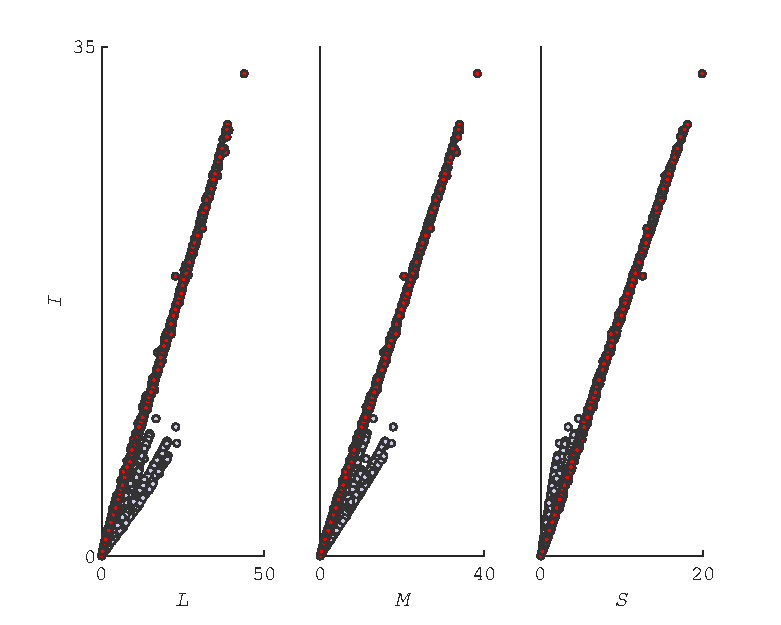
\includegraphics[max width=\textwidth]{figs/comp/melcomp_1/correlationBetweenLevel1Sigs.pdf}
%     \caption{The relationship between melanopic power (analogous to a tristimulus value but calculated using the spectral sensitivity of melanopsin). Red points indicate signals computed directly from the spectral power distribution, grey points represent values of computed colorimetry for objects under illuminants.  The traditional tristimulus values show a very strong correlation for illuminant-only values. It is not particularly easy to see here, but each surface is represented by a roughly straight line of grey points at slightly different angles.}
%     \label{fig:tristimCorrelation}
% \end{figure} 

% It should be noted that there was very high correlation between each signal. This is shown in Figure \ref{fig:tristimCorrelation} and the correlation table below. This can be considered as corresponding to the high importance of the first principal component of the spectral measurements in this dataset. Put another way, a sensor with almost any spectral sensitivity could be used to estimate the general magnitude of the daylight. The discussion of principal components will be returned to under melcomp\_3.

% \begin{lstlisting}
% corr(LMSI)
%     1.0000    1.0000    0.9993    0.9998
%     1.0000    1.0000    0.9995    0.9999
%     0.9993    0.9995    1.0000    0.9999
%     0.9998    0.9999    0.9999    1.0000
% \end{lstlisting}


